\chapter{Mise en place d'un modèle de formation et d'évolution stellaire}
\label{sec:etoiles}

Dans les parties précédentes nous avons présenté quelles étaient les différentes physiques à l’œuvre dans les simulations de la réionisation et la façon dont elles sont modélisées numériquement.
Il manque encore une composante essentielle au problème qui est la modélisation des sources de rayonnement ionisant.
Comme nous avons vu en introduction (cf section \ref{sec:introreio}), il existe deux types de sources, les étoiles et les quasars.
Dans la suite de cette étude, je n'ai considéré que la partie stellaire sans me préoccuper des quasars.
Dans cette section je vais présenter le modèle de formation stellaire que j'ai développé, ainsi que son implémentation dans EMMA et sa calibration.
%Dans ce modèle, la formation stellaire a lieu en trois temps.
%L'objectif de cette section est d'exposer le modèle de sources que j'ai développé, implémenté et calibré.
Nous allons définir les différentes phases de la vie d'une étoile, et ses différentes évolutions possibles.
%Il faut d'abord localiser les régions de formation, puis calculer la quantité d'étoiles à former, et enfin former les particules.
Nous verrons comment les contraintes imposées par les échelles cosmologique que l'on cherche à étudier vont imposer certains choix au niveau numérique.
Une attention particulière sera mise sur la modélisation des supernovæ, puisque une étude comparative entre deux modèles d'injection d'énergie suivra.
Lors de cette comparaison, il s'est avéré que dans nos modèles, les supernovæ étaient capable de réguler le \ac{SFR}, sans changer l'histoire de la réionisation.
Ce chapitre fait écho à la publication présentée en annexe \ref{pap:feedback}.
%\section{Les différentes phases de la vie d'une étoile}
%
%L'objectif est ici de définir les différentes phases de la vie d'une étoile.
%Nous allons aborder sa naissance, sa vie et sa mort de manière générale dans un premier temps.
%Et nous verrons ensuite l'implémentation de ces trois phases dans EMMA.

%\section{Modèle sous grille et population stellaire}

\section{Considérations de résolution}
%En fonction des echelles de travail, nous considererons soit les etoiles individuelles soit une population stellaire.

Une des difficultés majeures dans les simulations de la réionisation, est l'impossibilité d'obtenir des résolutions suffisantes pour suivre la formation des sources de rayonnement individuellement, tout en simulant un volume suffisamment important.
%Il existe toujours ce conflit en réionisation entre simuler des grands volume, et obtenir la meilleur résolution possible.
Actuellement les simulations de l'\ac{EoR} capables de suivre un volume d'Univers de l'ordre de $(100Mpc)^3$ atteignent un résolution de l'ordre du kilo-parsec.
Or les échelles de formation stellaire sont de l'ordre de l'unité astronomique, soit un facteur $\approx 10^8$ plus petit.
Il est donc actuellement impossible de résoudre les deux extrêmes du spectre d'échelles spatiales.
%de suivre la formation des étoiles individuellement.
Il est nécessaire de créer un modèle qui va tenter de prendre en compte au mieux la physique non résolue.
Ce type de modèle est appelé modèle \textit{sous-grille}.
Dans le cas présent le modèle sous-grille consiste à transformer une partie du gaz en particule stellaire, cette particule ne représentant pas une étoile mais une population stellaire de manière statistique.
%On appelle ces particules des particules puits.
Toute la difficulté du modèle de formation stellaire sera de déterminer la façon dont est réalisée cette conversion.
Malgré tout, nous verrons qu'il est possible d'obtenir un modèle statistiquement viable à grande échelle assez facilement.

% Un second type de modèle intervient au moment de l'explosion en supernovae.
% Les processus de diffusion de l'énergie libérée aux échelles plus petite que la grille sont complexe et il en résulte une série de paramètres libres assez conséquente.

%lien entre les différents solveurs en fonction du stade évolutif
%Les étoiles se trouvent aux centre de la simulation.
%En effet, créer une étoiles consiste a transformer une partie du gaz en particule.
%Cette particule sera ensuite gérée par le solveur Ncorps, et servira de source au solveur radiatif.
%Puis a la fin de sa vie, l'étoile va injecter de l'énergie dans le solveur hydrodynamique.
%Une particule stellaire va donc devoir interagir avec tout les solveurs du code.

%Seul la partie du spectre capable de ioniser l'hydrogène est considérée. E>13.6eV



\section{La formation stellaire}

\subsection{Critère de Jeans}

%lien avec la densité\\
%Formation dans l'H moléculaire mais pas dans les simu

Les étoiles se forment au sein de nuage de gaz, par effondrement gravitationnel.
Si les conditions sont réunies, cet effondrement ne s'arrête que quand les réactions thermonucléaires s'enclenchent et que le gaz forme une étoile.
En première approximation, un nuage de gaz s'effondre, si le temps de chute libre : 
\begin{equation}
t_{ff} =  \sqrt{\frac{3\pi}{32G\rho_g}} \propto \frac{1}{\sqrt{G \rho}},
\label{eq:tff}
\end{equation}
est inférieur au temps de réaction à une perturbation.
Considérant que cette perturbation est d'origine mécanique, le temps de réaction sera équivalent au temps de traversée du nuage par une onde sonore :
 \begin{equation}
t_{sound} = \frac{R}{c_s},
\end{equation}
avec $R$ la taille du nuage et $c_s$ la vitesse du son dans ce nuage.
Si le temps de réaction est plus long que le temps de chute libre
\begin{equation}
t_{ff} < t_{sound},
\end{equation}
alors le milieu n'a pas le temps de résister et le nuage s'effondre sur lui même.
$t_{ff}$ fait intervenir la densité, plus le milieu est dense plus il aura tendance à s'effondrer sur lui même.
Et de l'autre coté intervient aussi la vitesse du son $c_s$, elle même dépendante de la température $\left( c_s \propto \sqrt{T} \right)$ : plus le gaz sera chaud, plus le nuage va résister à son effondrement.
%\subsection{Population III}
%tres peu de ligne de refroisdissment
%étoiles plus grosse
% temps de vie court
%A haut redshift, au moment de l'apparition des premières étoiles, les métaux étaient très peu disponible (voir :\ref{sec:nucleosynthese_primordiale}).
%De ce fait, le gaz disposait de relativement peu de possibilité de refroidissement, menant à une température plus élevée.
%Les étoiles primordiales devaient donc être plus grosses que les étoiles de notre voisinage (plus de $100M_\odot$) \citep{2013RPPh...76k2901B}.
%Ce type d'étoiles est appelées étoiles de population III ou popIII.


%La nucléosynthèse primordiale a créer peu de métaux. 
%A haut redshift, les metaux etaient peu disponible.
%les métaux permettent une meilleur emmission radiative, et donc un meilleur refroidissent.
%si le refroidissment est meilleur, l'equilibre hydrostatique penche an faveur de plus grosse étoiles.
%POPIII, IMF top Heavy, étoiles  primordiales
%
%plus un étoiles est grosse, plus son spectre sera énergétique et plus la portion de spectre ionisant sera important.




\subsection{Localisation des zones de formation stellaire}

Il est admis que les étoiles se forment dans les nuages d'hydrogène moléculaire (voir eg \cite{krumholz_universal_2012}).
Ces nuages se trouvent eux même dans des zones suffisamment denses pour que des molécules puissent se former.
En pratique dans EMMA, la physique de l'hydrogène moléculaire n'est pas encore prise en compte, et les zones autorisées à former des étoiles sont localisées à l'aide d'un seuil en densité.
Toutes les cellules plus denses qu'un certain seuil sont autorisées à créer des particules stellaires .

%Seuil en densité \\
\begin{equation}
	flag = 
  \begin{cases}
      True, & \text{if } \rho > \rho_{thresh}\\
      False,              & \text{otherwise}
  \end{cases}
\end{equation} 

Ce type de critère est utilisé par la grande majorité des codes de simulations cosmologiques \citep{kay_including_2002}.
Cette densité de seuil $\rho_{thresh}$ peux être définie arbitrairement, et comme toute densité, elle est dépendante de la résolution.
De plus il en possible de définir une densité en unités physiques ou en unités comobiles (voir section \ref{sec:supercomobil}).
Un seuil en densité physique sera plus représentatif de se qui se passe réellement.
Mais à haut redshift, la densité était importante en tout points, et un seuil en unités comobiles est utile pour limiter l'apparition des premières étoiles à un redshift donné.
En pratique on pourra définir ces deux seuils, et le seuil final sera le plus contraignant des deux.

%TODO figure du seuil en fonction du redshift

\begin{equation}
	\rho_{thresh} = max\left(  \delta_{in} \bar{\rho}, \rho_{in} a^3 \right)
\end{equation} 

ou $\delta_{in}$ et $\rho_{in}$  sont respectivement les paramètres de surdensité et de densité physique.
$\delta_{in}$ est exprimé en unité comobile et est donc constant dans le temps en unités du code,
 $\rho_{in}$ est exprimé en unités physiques (en atomes par mètre cube), sa valeur évolue dans le temps du point de vue des unités du code (cf section \ref{sec:supercomobil}).

% determination de la valeur de 55\\ 
%TODO quells valeurs sont prisent et pourquoi?

\subsection{La loi de Schmidt-Kennicut}
\label{sec:schmidt-kennicut}
 %conversion densité surfacique vers densité 3D\\
%rho 1.5\\
%temps de free fall\\

Maintenant que nous avons défini où former des étoiles, il nous faut en calculer la quantité à former.
\cite{1959ApJ...129..243S} propose que le \ac{SFR} d'une galaxie évolue comme une fonction de la densité de gaz dans cette galaxie, et plus précisément comme une loi de puissance.
\cite{1998ApJ...498..541K} mesure cette loi pour les galaxies extérieures en fonction de leurs densité surfacique observée.

Cette relation, nommée loi de Schmidt-Kennicut a la forme :
\begin{equation}
\Sigma_{SFR} = (2.5 \pm 0.7) \times 10^{-4} \left( \frac{\Sigma_{gas}}{1 M_\odot pc^{-2}} \right)^{1.4 \pm 0.15}
\end{equation}

Il est toutefois nécessaire de mentionner que ce modèle n'est valable qu'aux échelles de l'ordre du kiloparsec. % et que l'utilisation de résolution plus fine nécessitera l'introduction de physique supplémentaire. 

%Il propose ensuite 
%
%a utilisé un modèle de galaxie pour dé-projeter la densité surfacique observée et ainsi déterminer une loi qui lie le \ac{SFR} à la densité volumique de gaz.
%
%\begin{equation}
%SFR \propto \rho ^{\alpha},
%\end{equation}

Le taux de formation stellaire s'exprime généralement en $M_\odot \cdot cMpc^{-3} \cdot yr^{-1}$  
Ce qui est homogène à une densité divisée par un temps.
En pratique on divisera $\rho_g$ la densité locale de gaz par le temps de chute libre (equation \ref{eq:tff}), qui est en théorie le temps nécessaire à un nuage de gaz pour s'effondrer si il n'y avait aucune résistance.
Au final, le \ac{SFR} prend la forme:
\begin{equation}
	SFR = \epsilon_{sf} \frac{\rho_g}{t_{ff}} \propto \rho_g^{1.5}
    \label{eq_sfr}
\end{equation}
avec  $\epsilon_{sf}$ le paramètre d'efficacité de formation stellaire.
Il est également possible de considérer le temps caractéristique de formation stellaire:
\begin{equation}
t_{sf} =  \frac{t_{ff}}{\epsilon_{sf}},
\end{equation}


Observationellement, la formation stellaire est relativement inefficace et $t_{sf}$ est de l'ordre de quelques milliards d'années menant à un $\epsilon_{sf}$ de l'ordre du \% \citep{krumholz_universal_2012}.
Ceci est dû à des phénomènes complexes comme la turbulence ou les champs magnétiques qui ont une importance prépondérante aux échelles de l'unité astronomique (voir par exemple \cite{2015MNRAS.450.4035F}).

%Ce qui signifie que la formation stellaire est relativement inefficace.

\subsection{Implémentation}

A partir du taux de formation, on obtient la masse de gaz à convertir en étoiles dans chaque cellule en multipliant par $dv$ le volume de la cellule en question et $dt$ le pas de temps entre deux passage dans la fonction de formation stellaire:
\begin{equation}
	M_{star} = SFR \cdot dv \cdot dt .
\end{equation}

%resolution en masse\\
Nous avons donc à ce stade la masse totale de gaz à convertir en étoile.
Il devient rapidement coûteux de générer pour chaque cellule éligible, et à chaque pas de temps, une nouvelle particule stellaire (le nombre de particules peut rapidement exploser).
Nous adoptons une approche probabiliste.
Nous définissons une masse d'étoiles $m_{star}$ qui correspondra à notre "quanta stellaire".
Toutes les étoiles auront donc la même masse et cette masse est calculée d'une manière comparable à celle d'une particule de matière noire.
La masse d'une étoile correspond à la masse moyenne de gaz dans une cellules d'un certain niveau :
\begin{equation}
 m_{star} = M_{DM} \frac{\Omega_b}{\Omega_m}\cdot 2^{-3L},
\end{equation}
où $L$ peux varier du niveau de base à niveau plusieurs niveaux raffinés.

Le nombre de quanta à ajouter est ensuite tiré aléatoirement dans une loi de Poisson \citep{rasera_history_2006}.
\begin{equation}
	P(N) = \frac{\lambda^N}{N!} e^{-\lambda}
\end{equation}

Où $\lambda$ correspond au nombre de particules moyen à créer dans la cellule :
\begin{equation}
\lambda = \frac{ M_{star}}{m_{star}}
\end{equation}
On obtiendra au final $N_{star}$ le nombre de quanta de masse d'étoiles à créer.
%Étant donné le grand nombre de tirages cette loi est en moyenne valide.

En pratique j'ai implémenté deux méthodes de transformations.
Si  $N_{star}>1$ il est possible de créer : 
\begin{itemize}
\item  $N_{star}$ particules aillant chacune une masse  $m_{star}$.
\item une seule particule de masse  $N_{star} \cdot m_{star}$.
\end{itemize}

Dans le premier cas le nombre de particules sera plus élevé et la résolution stellaire meilleure, mais en contrepartie le coût numérique sera plus important.
Le choix de la méthode est laissé à l'utilisateur et dépend de la situation.
Dans tous les cas la masse est conservée et la quantité de masse convertie est limitée au maximum à 90\% de la masse totale gaz de initialement présente dans la cellule, pour éviter que la formation stellaire ne puisse vider la totalité du gaz de la cellule.


%En pratique la création d'une particule stellaire consistera a 
%\begin{itemize}
%\item prendre dans la réserve, une nouvelle particule %un maillon de la liste chainée
%\item ajouter ce nouveau maillons a la liste chainée de particule de la cellule.
%\item initialiser cette nouvelle particule avec : 
%\begin{itemize}
%\item un état
%\item un temps de création
%\item une vitesse 
%\item une masse
%\item un identifiant
%\end{itemize}
%\end{itemize}

%TODO resolution masse stellaire
%TODO conservation de la masse

\subsection{Quelques détails techniques}
En pratique la création d'une particule stellaire consistera à prendre une nouvelle particule vierge dans la réserve (cf section \ref{sec:PART}), ajouter ce nouveau maillon à la liste chaînée de particule de la cellule et initialiser cette nouvelle particule.

\begin{itemize}

\item La position sera choisie aléatoirement au sein de la cellule.
La vitesse correspondra à la vitesse du gaz au moment de leur création à laquelle on ajoutera une composante avec une direction aléatoire et une amplitude aléatoirement comprise entre $\pm c_s$ la vitesse du son dans la cellule \citep{rasera_history_2006}.
Ceci évitera à une cellule donnée de former, sur plusieurs pas de temps d'affilé plusieurs particules aillant toutes la même direction et la même vitesse, formant alors un effet de "collier".
%Dans cette configuration, il est possible qu'une zone dense forme des étoiles pendant plusieurs pas de temps d'affilés.
%Or au moment de leurs création les étoiles passe d'une physique collisionnelle (celle du gaz), à une physique non collisionnelle
%%Pour éviter les effets de "collier", à cette vitesse sera ajoutée 
%Pour minimiser cette effet on ajoutera à la vitesse initiale une composante, aillant u

\item Contrairement aux particules de matière noire, les étoiles doivent conserver l'information sur leur instant de création.
%On associera un instant de création à la particule stellaire et non un age, pour ne pas avoir à remettre à jour cette valeur à chaque pas de temps.
%Pendant les analyses post-simulations, on prendra garde à définir l'age des étoiles comme étant l'instant associé au snapshot courant moins l'instant de création de la particule.


\item Il est utile d'associer un identifiant unique aux nouvelles particules pour pouvoir suivre leur évolution et les retrouver entre les différentes sorties.
La technique la plus simple est d'associer la valeur d'un entier que l'on incrémente à chaque création d'une nouvelle particule.
Du fait de la parallélisation cette incrémentation demande des communications à chaque création de particule.
Pour minimiser les communications, la pratique retenue consiste à former toutes les particules de toutes les processus, en leur assignant un identifiant caractéristique (eg -1) et d'assigner les identifiants finaux dans un second temps.
Une fois les particules créées, chaque processus compte son nombre de nouvelles particules et le transmet aux autres, ce qui permet d'allouer une plage d'identifiants par processus, et ainsi allouer les identifiants finaux.
\end{itemize}

%\begin{figure}
%        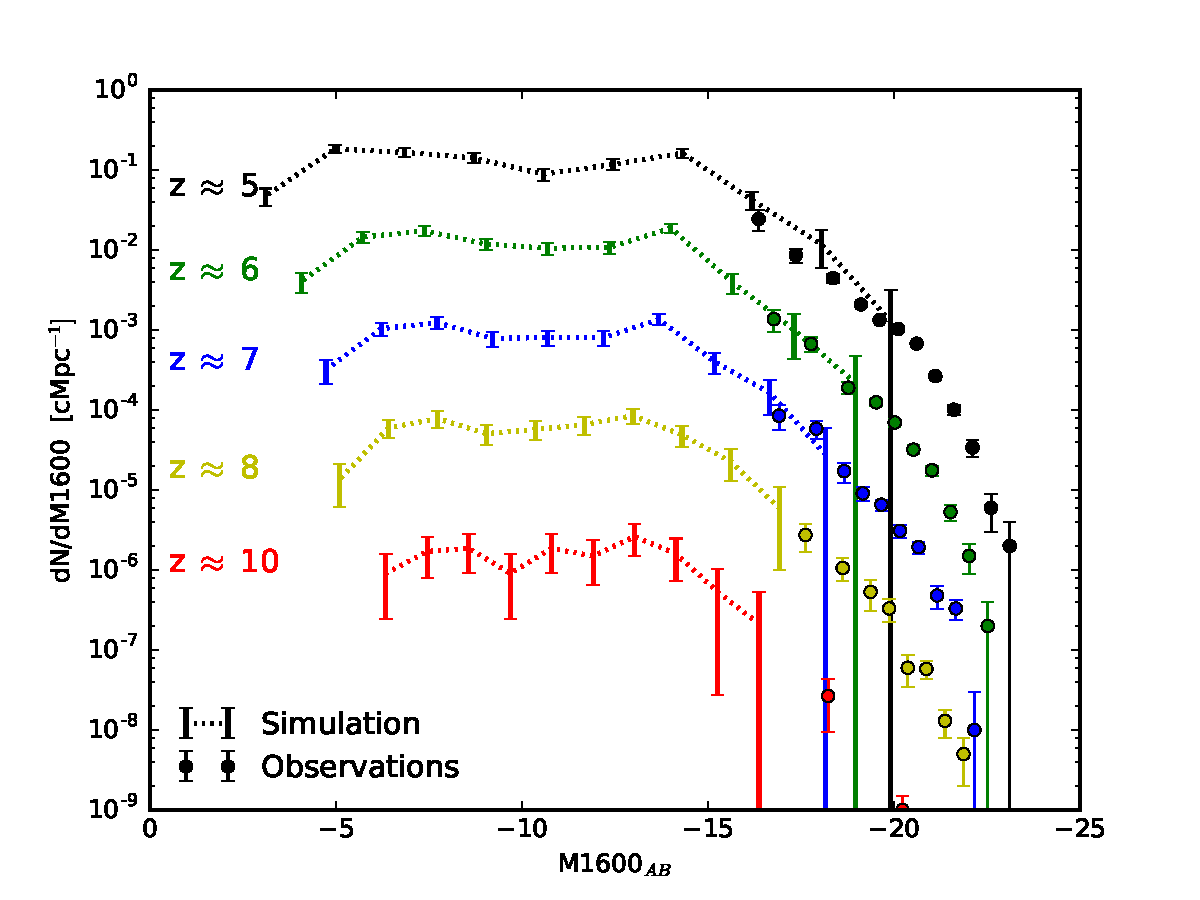
\includegraphics[width=.95\linewidth]{img/02/luminosity_function.pdf}
%        \caption{Fonction de luminosité dans la bande $M_{1600}$.
%}
% 		\label{fig:test_SFH}
%\end{figure}

%Des test plus poussés seront développés plus loin.

%\clearpage
\section{La phase radiative}
\label{sec:etoilerad}

%%\subsection{Vie}
%%le diagram HR
%
%Une fois le nuage de gaz effondré et les réactions thermonucléaires amorcées, l'étoile amorce sa séquence principale.
%C'est la phase qui représente la majeure partie de la vie d'une étoile.
%Elle consiste en un équilibre hydrostatique entre gravitation et pression interne, maintenue par les réactions de fusion nucléaire.
%L'étoile va consommer son hydrogène pour résister à l'effondrement gravitationnel, il en résultera une formation d'hélium.
%%develloper le cycle proton proton ?
%L'équation simplifié du processus de fusion, appelé cycle proton-proton (PP) est :
%\begin{equation}
%4p \leftrightarrow He^4 + 2e^+ + 2\nu + E.
%\end{equation}
%
%Plus une étoile est grosse plus le taux de réaction doit être élevé pour lutter contre la gravité.
%Il en résulte que les grosse étoiles sont plus énergétique, et émettent donc plus de rayonnement ionisant.
%En contre partie, ce taux de réaction élevé mène à une durée de vie plus courte.
%Du fait de leurs masses, les popIII, émettaient un fort rayonnement ionisant, et avaient une vie relativement courte.
%
%%materiaux de base est l'hydrogene\\
%%plasma donc hydrogène ionisé 
%


\subsection{Modèle de population stellaire}
\label{sec:staburst}
%Pour modeliser 
%paramètre d'entrée
%sorties

Une fois les étoiles formées, il est nécessaire de les faire rayonner.
Dans notre modèle, une particule stellaire ne correspondra pas à une étoile unique mais sera représentatif d'une population.
Les étoiles d'une population ayant des masses et des évolutions différentes, l'émission résultante sera la somme des contributions individuelles.
Pour déterminer quel est le lien entre age, masse et luminosité d'une particule stellaire on utilisera un modèle de population stellaire.
Il existe différent modèles dédiés à cette tache, on peut citer entre autres :

\begin{itemize}
\item Starburst99 \cite{leitherer_starburst99:_1999} 
\item \cite{2003MNRAS.344.1000B}
\item FSPS \cite{2009ApJ...699..486C}
\end{itemize}

À partir d'informations caractéristiques d'une population stellaire, comme sa masse totale, sa fonction de masse initiale \ac{IMF} (voir cection \ref{sec:imf}) ou sa métallicité, ces modèles retournent un spectre d'émission en fonction du temps (cf Fig \ref{fig:spectre_starburst}).
Le choix a été fait d'utiliser Starburst99, car en plus des spectres, il retourne plusieurs informations utiles au modèle comme l'énergie et la masse injectées par les supernovae (section \ref{sec:sncali}).
De plus Starburst99 possède une interface web rendant son utilisation aisée.

\begin{figure}
        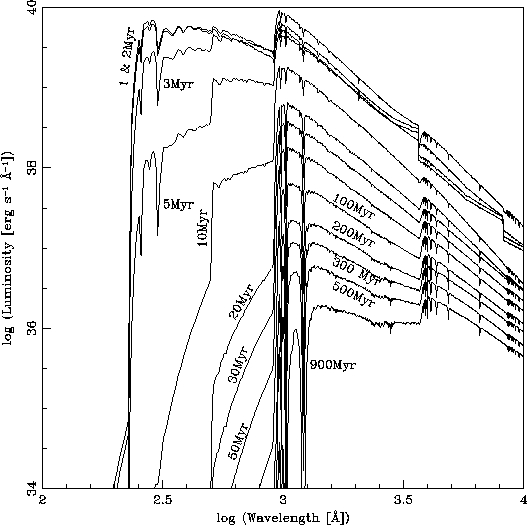
\includegraphics[width=.95\linewidth]{img/03/spectre_starburst.jpg} 
        \caption[Spectres Starburst99]{Spectre d'émission d'une population stellaire généré par Starburst99.
        Ici avec les paramètres : $M_{pop}=10^6 M_\odot$, \ac{IMF} de Salpeter ($\alpha=2.35$ et intégration de 1 à 100 M$_\odot$ 
 		\label{fig:spectre_starburst}}
\end{figure}

%injection d'énergie dans le solveur radiatif, ok mais combien?\\
%calibration energetique et Starburst99\\

%J'ai commencé mes calibrations avec une \ac{IMF} de Salpeter, mais il s'est vite avéré que les sources n’émettaient pas assez de photons ionisant et que les boites n'arrivaient pas a reioniser.
%La majorité des simulations que j'ai réalisées ensuite utilisent une \ac{IMF} Top-Heavy.


À partir des spectres obtenus avec Starburst99 (cf section \ref{sec:staburst}), nous allons ne garder que la partie capable de ioniser l'hydrogène (toutes les longueurs d'onde plus courte que 912$\AA$) :

\begin{equation}
E_{ion (t)} = \int_{13.6eV}^{+\inf} h \nu_{(t)} d\nu
\end{equation}

En divisant l'énergie totale obtenue à partir de cette intégration par l'énergie moyenne des photons obtenue à partir des spectres (cf section \ref{sec:groupedephotons}), on obtient l'évolution du flux de photons ionisant, présentée sur la figure \ref{fig:flux}.
\begin{figure}
        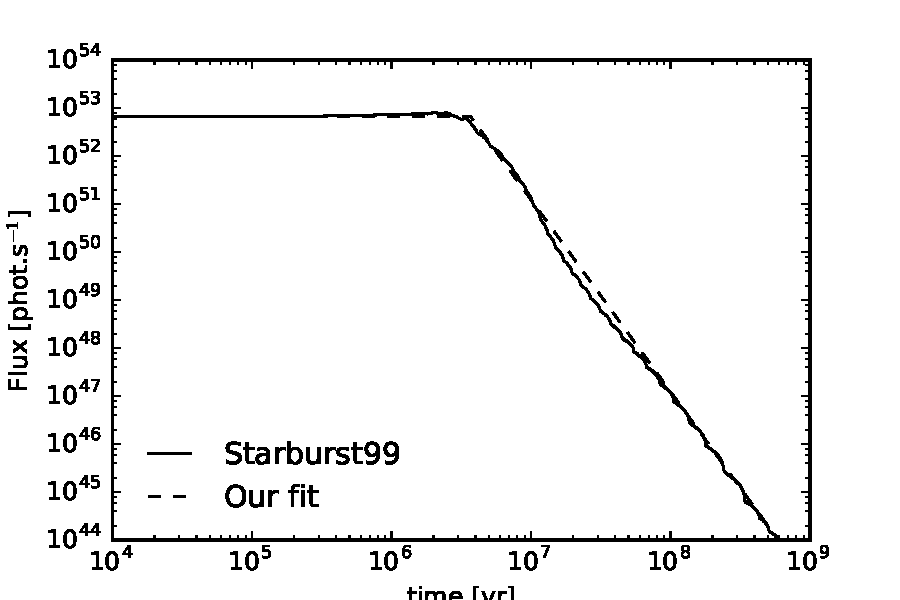
\includegraphics[width=.95\linewidth]{img/03/flux.pdf} 
        \caption[Émissivité ionisante]{Émissivité ionisante intégrée en fonction du temps pour une population de $M_{pop}=10^6 M_\odot$.
        La population présente deux phases d'émission, une phases constante suivie d'une rapide décroissance.
 		\label{fig:flux}}
\end{figure}
Le profil obtenu présente un plateau d'émissivité constante suivie d'une rapide décroissance.
Ce profil peut être raisonnablement approximé par:

\begin{equation}
    S = 
\begin{cases}
    S_0 ,         & \text{if } t < t_{life}\\
    S_0.t^{-4},   & \text{if } t_{life} \leq t < 100t_{life} \\
    0,   & \text{if } 100t_{life} \leq t
\end{cases}
\end{equation}

où $t_{life}$ est définis comme étant l'age de la population au moment de changement de régime.
Par la suite nous utiliserons la valeur de $t_{life} = 3.7$ Myrs.
Étant donnée la rapide décroissance en luminosité, les étoiles sont arbitrairement éteintes après $100 \cdot t_{life}$.

Le flux obtenu correspond au flux d'une population de $10^6M_\odot$, ces valeurs seront pondérées au prorata de la masse de la particule stellaire : une particule de $10^5M_\odot$ émettra simplement 10 fois moins de photons ionisants qu'une population de $10^6 M_\odot$.

Cette émissivité sera ensuite pondérée par $f_{esc}$ un paramètre d'efficacité et $S'$ l'énergie effectivement rayonnée dans la simulation ne sera qu'une partie de $S$ l'énergie totale disponible : $S' = f_{esc} \cdot S$.
Ce paramètre libre reflète l'impact d'une grande partie de la physique sous grille, sur le rayonnement.
En effet, nous ne résolvons pas certains processus, comme par exemple l'absorption par la poussière, qui va empêcher le rayonnement de sortir de l’environnement de la population.
Ce paramètre est analogue à une fraction d'échappement intrinsèque et ne doit pas être confondu avec la fraction d'échappement des galaxies que nous aborderons par la suite (voir section \ref{sec:fesc}).

%Il nous reste encore à caractériser le type de photons à émettre.
%La gestion des groupes de photons a été abordée dans la section \ref{sec:groupedephotons}, nous ne travaillerons par la suite qu'en émission mono-groupe.
%Les caractéristiques des photons émis dans le cas d'une \ac{IMF} Top-Heavy sont présentés sur la table \ref{tab_photon}.

%\begin{table}
%\begin{tabular}{l l }
%	$<h\nu>$	&  $23.42$ eV \\
%	$\alpha_e$	&  $2.35.10^{-22}$ m$^2$ \\
%	$\alpha_i$	&  $1.82.10^{-22}$ m$^2$ \\
%\end{tabular}
%\caption[Propriété des photons]{Propriété des photons émis par les sources.
%Ces valeurs ont été calculées à partir des spectres obtenus avec Starburst99.
%\label{tab_photon}}
%\end{table}

\subsection{Fonction de masse initiale}
\label{sec:imf}

Un paramètre central dans les modèles de populations stellaires est l'\ac{IMF}, qui exprime la probabilité $A$ de former une étoile d'une certaine masse $m$ dans une population.
%Les étoiles naissent en groupe, et toutes ne sont pas identique.
%L'\ac{IMF} caractérise cette diversité, et 
Elle prend généralement la forme d'une loi de puissance :
\begin{equation}
A_{(m)} = a_0 \cdot m^{-\alpha},
\end{equation}
pouvant être caractérisée par des valeurs de $\alpha$ différentes, parfois avec plusieurs intervalles.
Parmi les \ac{IMF} plus connues il y a :

\begin{itemize}
\item \cite{1955ApJ...121..161S}
\item \cite{1979ApJS...41..513M}
\item \cite{2001MNRAS.322..231K}
\item \cite{2003PASP..115..763C}
\end{itemize}


%Comme nous l'avons abordé plus haut, les étoiles de population III avaient tendance a être très massive.

Certains travaux \citep{2003MNRAS.344L...7C,2013RPPh...76k2901B} suggèrent que lors de la réionisation, la proportion d'étoiles massives était importante, j'ai donc utilisé par la suite une \ac{IMF} Top-Heavy avec les caractéristiques suivantes :

\begin{equation}
	\alpha = 
  	\begin{cases}
	1.3 & si 0.1 < m/M_\odot \leq 0.5\\
	2.3 & si 0.5 < m/M_\odot \leq 1 \\
	1.6 & si 1   < m/M_\odot \leq 100 \\
	\end{cases}
\end{equation} 

De plus, les premiers tests de calibrations, %TODO ref
ont été réalisés avec une \ac{IMF} de Salpeter, il s'est avéré que la quantité de rayonnement ionisant était trop faible, même en utilisant une fraction d'échappement de $100$\%.
L'utilisation d'une \ac{IMF} Top-Heavy à permis d'augmenter la proportion d'étoiles massives et d'augmenter la quantité de rayonnement ionisant disponible, permettant ainsi l'utilisation d'une $f_{esc}<1$.

%: difficulté a reioniser avec Salpeter -> passage a top heavy -> justification 
%Fonction de masse IMF Top Heavy


\subsection{Quelques détails techniques}

En pratique, il faudra calculer l'émissivité sur toute les cellules de la grille.
Cette opération est simplifiée par l'utilisation de la liste chaînée de particules (cf section \ref{sec:PART}).
En effet, on passera en revue toutes les cellules, et pour chaque cellules on passera en revue toutes ses particules.
On testera alors si une particule est une étoiles (la liste chaînée contient également les particules de matière noire), et si cette étoile est dans un stade où elle émet de l'énergie ionisante.
Si c'est le cas, on calculera son émissivité et on injectera cette énergie sous forme de source dans l'équation \ref{eq:densite_energie}.
%Le calcul de $\dot{N}_\nu^*$ sera effectué dans toutes les cellules.




%TODO intégration de l'énergie et de la section efficace


%We found a mean energy of $<h\nu> = 23.42$ eV,
%an energy weighted cross section of
%$\alpha_e = 2.35.10^{-22}$ m$^2$
%and a number weighted cross section of
%$\alpha_i = 1.82.10^{-22}$ m$^2$


%Masse de la population\\
%produit en croix pour correspondre a la masse dans simu\\
%integration seulement sur energy ionisante\\
%
%Multigroupe frequence\\
%multigroup temporel\\


\section{Les supernovæ}

%Il a fallut trouver un mécanisme d'introduction d'énergie dans le gaz.
%Les supernoavae ont été proposées comme mécanisme.

Les supernovae ont été introduites dans les simulations cosmologiques pour réduire l'effondrement du gaz sur lui même.
Sans l’introduction d’énergie dans le gaz par les supernovæ, le gaz s’effondre de manière importante et cela mène à un taux de formation stellaire trop important par rapport à ce qui est observé ainsi qu’a des tailles, rotation et géométrie des disques galactiques non conformes. Ce problème est connu sous le nom de "overcooling problem" \citep{2003ApJ...599...38B, 1992A&A...264..365B,2003ApJ...599...38B, 1992A&A...264..365B}


%Sans l'introduction d'énergie dans le gaz par les supernovæ, le gaz s'effondre de manière importante et cela mène à un taux de formation stellaire trop important par rapport à ce qui est observé.
%Ce problème est connu sous le nom de "overcooling problem" \citep{2003ApJ...599...38B, 1992A&A...264..365B}.
%%L'objectif est de "casser" les structures pour diminuer les surdensités et limiter la formation stellaire.
%Également, \citep{2000ApJ...538..477N} ont proposé d'introduire les supernovae dans les simulations pour reproduire la taille et la géométrie des disques galactiques observée.

Dans cette section faisant également référence à la publication présentée en annexe \ref{pap:feedback}, nous allons aborder la modélisation des supernovæ dans les simulations cosmologiques.
Je présenterai deux des modèles que j'ai implémenté, ainsi que les tests numériques qui vont permettre de les valider.
%Nous verrons que ces modèles sont équivalent dans un contexte idéal mais divergent lors de l'introduction de la physique du refroidissement.
%Nous aborderons également la problématique de la calibration de ces modèles.


%\subsection{Le modèle théorique}
%Il existe principalement deux événement pouvant mener a un explosion de supernovæ : 
%
%\begin{itemize}
%\item soit l'étoile est a l'origine suffisamment massive (plus de 8Mo) pour s'effondrer a la fin de sa vie.
%\item soit l'étoile n'est pas suffisamment massive (elle va donc mourir en naine blanche) mais dispose de suffisamment de matière a proximité (généralement étoiles double ou le compagnon pas en phase géante rouge) pour que sa masse augmente avec le temps.
%la matière accreté va faire passer la masse de cette étoile au dessus de la limite.
%\end{itemize}
%
%Les étoiles de plus de 8mo exploses en SN en injectant 1e51 erg dans le milieu\\
%Cette injection limite fortement la formation stellaire dans le milieu.\\
%modèle sous grille\\


\subsection{La mort d'une étoile massive}
\label{sec:snmort}

%Arrivé à un certain taux de consommation d'hydrogène, les réactions protons-protons ne sont plus suffisantes, l'équilibre entre la gravité et la pression est rompu et l'étoile s'effondre sur elle même.
%A la fin de sa vie, une étoile a consommée la plus grande partie de son hydrogène disponible.
%L'équilibre entre la gravité et la pression est rompu, ce qui mène à une augmentation de la pression interne.
%% Géante rouge ?
%Cette augmentation de la pression amorce une nouvelle série de fusions nucléaires, qui va consommer des éléments plus lourds que l’hydrogène, tel le carbone, l'azote ou l'oxygène (cycle CNO) jusqu'au fer où le processus s'arrête.
%A ce stade, les couches externes de l'étoiles se contracte rapidement, et rebondissent sur le noyau de fer.
%Une fois arrivé au Fe, il devient coûteux de continuer a fusionner des éléments car Fe est le plus stable.

%Il existe principalement deux types de supernovæ : 
%\begin{itemize}
%\item Les types I où l'étoile n'est pas assez massive à la base pour permettre l'explosion en supernovae.
%Ce sont généralement des étoiles binaires où une des deux étoiles accrète une partie de son compagnon, ce qui mène au passage au dessus de la masse limite et provoque l'explosion.
%\item Les types II : les étoiles de plus de $8 M_\odot$ sont assez massives pour exploser en supernovæ sans avoir besoin de masse supplémentaire.
%\end{itemize}


%Après l'explosion de la supernova, le cœur subsiste et en fonction de sa masse, plusieurs scénario d'évolution sont possibles.
%En fonction de la masse de l'étoiles, le résidu peux devenir une naine blanche, une étoile à neutron ou un trou noir.
%Dans tout les cas, 


%\begin{itemize}
%\item Naine blanche %(maintenue par le pression de dégénérescence des électrons)
%\item Étoile a neutron %(pression de dégénérescence des neutrons)
%\item Trou noir %(singularité)
%\end{itemize}



À la fin de la vie d'une étoile, l'équilibre entre la gravité et la pression est rompu et l'étoile s'effondre sur elle même.
Les étoiles de plus de $8 M_\odot$ explosent alors en supernovae et injectent énormément d'énergie dans le milieu, de l'ordre de $10^{51}$ erg par explosion. 

%Pendant l'explosion, l'énergie libérée est suffisamment importante pour amorcer la formation d'éléments plus lourds que le fer.
%Ces éléments, ainsi que ceux formés pendant la vie de l'étoile vont être expulsés, et vont participer à l'enrichissement du milieu.
%Les propriétés physico-chimiques du gaz environnant vont alors évoluer et cela va avoir des conséquences sur la formation des prochaines générations d'étoiles.
%Après l'explosion, le cœur subsiste et continue à interagir gravitationnellement avec son environnement.

Après l'explosion d'une supernovae, il en résulte une onde de choc qui va se propager dans le milieu environnant.
L'évolution du front d'onde a lieu en plusieurs phases \citep{1998ApJ...500..342B,1974ApJ...188..501C}, on en distinguera principalement deux : 

\begin{itemize}
\item Expansion adiabatique.
Dans la phase d'expansion adiabatique, l'énergie cinétique est conservée, le choc est violent et le gaz n'a pas le temps de perdre de l'énergie par rayonnement.
Dans cette phase, le front d'onde est suffisamment rapide pour que la dissipation d'énergie par rayonnement soit négligeable.
%C'est par exemple le cas du test de Sedov.

\item Snowplow.
Dans la phase snowplow, le choc a suffisamment ralentis pour que le gaz commence à dissiper de l'énergie par rayonnement.
Dans ce cas, il se forme un bourrelet de compression dans lequel le gaz est poussé, comme dans le cas d'un chasse neige. 
Les pertes par rayonnement deviennent importantes et l'énergie cinétique n'est plus conservée.
\end{itemize}

%\subsection{Les Superbubbles}
%A la manière de la percolation des bulles de HII, les bulles de supernovae 

Dans les lieux de formation stellaire, les étoiles ne sont pas isolées, mais apparaissent ensemble au sein d'un même nuage de gaz.
L'effondrement gravitationnel du nuage mène à créer une génération d’étoiles en un cours laps de temps.
Toutes ces étoiles vont mourir dans un court délai et les différentes supernovæ vont injecter de l’énergie dans le milieu en même temps.
Les différentes ondes de chocs vont se cumuler et la résultante va mener à la création d'une bulle de gaz chaud pouvant englober les galaxies.
On appelle ces régions des superbubbles (voir eg \cite{1986PASJ...38..697T,keller_superbubble_2014,2017ApJ...834...25K}).

%\subsection{Considérations d'échelles}
La façon de gérer les supernovæ sera donc fonction de l'échelle que l'on considère.
Dans des simulations détaillées de galaxies, il sera nécessaire de résoudre la phase adiabatique des explosions d'étoiles individuelles. %TODO ref simu de galaxie zoom
Dans les simulations cosmologiques de la réionisation qui nous intéresses ici, l’intérêt sera plus porté sur la phase snowplow des superbubbles.

%\subsection{ Différentes implémentations existantes}
%\subsubsection{Navaro and white}
%\subsubsection{Stinson et al}
%\subsubsection{dubois et Teyssier}
%Utilisation de particule fantômes pour simuler les différentes phase
%
%\subsubsection{Dalla Veccia et Schaye}
%Modèle probabiliste, injection d'énergie seulement si l'énergie est suffisante pour générer un mouvement suffisant.

\subsection{Mes Implémentations}
\label{sec:SNmodel}


Voyons a présent comment modéliser ces explosions.
Je vais présenter dans les prochaines sections deux modèles d'injection d’énergie dans le gaz que j'ai implémenté dans EMMA.

\subsubsection{Modèle thermique}
Le modèle thermique consiste à injecter l’énergie de l'explosion sous forme d’énergie interne:
\begin{equation}
E^{t+1} = E^t + E_{SN},
\end{equation}
où $E_{sn}$ représente l'énergie apportée par les supernovae.
%Il existe 2 variables d’état liées à l’énergie interne : la pression et la température.
%Modifier l'une ou l'autre est équivalent et dans l’implémentation actuelle, 

En pratique le choix a été fait de travailler sur la pression, elle est modifiée de la manière suivante :

\begin{equation}
P^{0+} = P^{0-}  + E_{SN} \cdot  (\gamma-1)
\end{equation}
où $\gamma$ l'indice adiabatique du gaz.

L'injection d'énergie va donc résulter en une augmentation de la pression dans la cellule et le gaz sera mis en mouvement par conversion de l'énergie interne en énergie cinétique. 
L'avantage de cette méthode est que l'injection ne nécessite la modification que d'une seule cellule.
Cependant il est connu pour avoir de fortes pertes de d'énergie dans le cas où le refroidissement est autorisé \citep{navarro_simulations_1993}. 

\subsubsection{Modèle cinétique}

Le modèle cinétique a pour objectif de court-circuiter le conversion entre énergie interne et énergie cinétique en modifiant directement cette dernière.
Il consiste à modifier directement la vitesse du gaz autour de l'explosion. % dans le but de shunter la conversion de l'énergie interne en mouvement.
%Ce type de model a été utilisé pour 
Il n'est plus possible ici de ne modifier qu'une seule cellule, et plus le nombre de cellules dont la vitesse sera modifiée autour de l'explosion sera important, meilleure en sera la sphéricité de l'onde choc.
Le choix a été fait de limiter le nombre de cellules utilisées à 8 correspondant à 1 oct de la structure \ac{AMR} d'\emma\ (voir figure \ref{fig:kin}).
Ceci à deux conséquences.
Premièrement la recherche de voisin est réduite à l'exploration de l'OCT parent de la cellule où a lieu l'explosion, le coût numérique est donc réduit à son strict minimum (voir section \ref{sec:voisins}).
Deuxièmement, un OCT ne peut pas être divisé entre les domaines, ce qui assure que l'explosion a lieu au sein d'un processus unique et permet d'éviter les communications.

En pratique l'énergie de l'explosion sera uniformément répartie sur les 8 cellules de l'OCT, ainsi chaque cellule recevra : 

\begin{equation}
e_{SN} = E_{SN}/8.
\end{equation}

Cette énergie est utilisée pour changer la vitesse du gaz de chaque cellule en utilisant : 

\begin{equation}
    \Delta \overrightarrow{v_{gas}} = \sqrt{\frac{2e_{SN}}{\rho_g.dV}} \overrightarrow{u},
    \label{eq_sn_direct}
\end{equation}

où les vecteurs $\overrightarrow{u}$ sont les directions radiales au centre de l'OCT présentés sur la figure \ref{fig:kin}.

\begin{figure}
        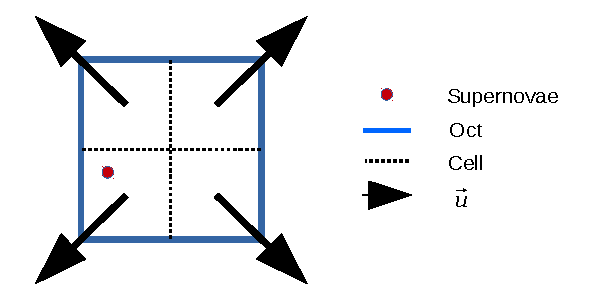
\includegraphics[width=.95\linewidth]{img/03/oct_kinetic.pdf} 
        \caption[Injection d'énergie cinétique]{Avec le modèle cinétique l'explosion a lieu au sein d'un OCT, et radialement au centre de celui ci.
 		\label{fig:kin}}
\end{figure}

\subsection{Retour de masse}
Les deux modèles présentés ont la possibilité de retourner de la masse dans le milieu environnant après l'explosion.
La totalité de la masse sera retournée dans une cellule dans le cas du modèle thermique, ou uniformément distribuée dans les 8 cellules de l'OCT dans le cas du modèle cinétique.
En pratique la densité de la cellule sera modifiée:
\begin{equation}
\rho^{0+} = \rho^{0-} + \frac{M_{SN}}{dV}.
\end{equation}
L’enrichissement en métaux n'est pas considéré actuellement, mais fait partie des améliorations planifiées.
%(cf section \ref{sec:snmort})
\subsection{Explosion de Sedov}
\label{sec:sedov}

%la dérivation des solutions du test de Sedov se trouve :
%chapitre 17 de Shu the physique of astrophysic Volume 2.\\

Dans le but de tester l'implémentation des différents modèles d'injection d'énergie, je les ai soumis au test de Sedov.
Ce test est utilisé pour tester le cas d'une explosion parfaite et présente l'avantage de posséder une solution analytique.
Il consiste à relâcher instantanément une quantité d'énergie $E_0$ dans un milieu homogène d'indice adiabatique $\gamma$, de densité $\rho_0$ et de pression $P_0$ (ou de température $T_0$).
Ce brusque changement dans l'état du système créer une discontinuité que le solveur va devoir gérer.
\cite{sedov_similarity_1959} a exprimé $r_{(t)}$ le rayon de l'explosion en fonction du temps  : 

\begin{equation}
r_{(t)}=\left( \frac{E_0}{\alpha \rho_0 }\right)^{1/5} t^{2/5}
\end{equation}

%TODO expression analytique du profil

\subsubsection{Évolution temporelle }

%parametre du test :
%rho=1
%p=1e-5
%v=0
%gamma=5/3

Ce premier test consiste à injecter l'énergie dans le milieu à l'aide de la méthode d'injection thermique dans une seule cellule et à suivre l'évolution du profil et de la position de l'onde de choc dans le temps.
%On s'assure alors que son profil et sa position sont correct 
%On calcul pour chaque cellule sa distance au centre de l'explosion, puis en utilisant un histogramme sur les rayons, pondéré par la valeur du champ que l'on veux analyser, on obtient rapidement le profil radial moyen.

La colonne de gauche de la figure \ref{fig:sedov_profil} présente les profils radiaux de densité, de pression et de vitesse radiale à trois instant différents, comparés à la solution analytique.
Le domaine est une grille régulière décomposée en $256^3$ éléments de calcul où le raffinement n'est pas autorisé.
On observe un très bon accord entre la simulation et la théorie, l'implémentation de la méthode d'injection d'énergie thermique est donc correcte et bien dimensionnée.

\subsubsection{Comparaison des modèles}

Le test présenté ici consiste à vérifier la validité de différentes méthodes d'injection, nous allons en comparer trois : 
\begin{itemize}
\item l'injection thermique dans une cellule,
\item l'injection thermique dans un cube de huit cellules,
\item l'injection cinétique dans un cube de huit cellules.
\end{itemize}

Les trois simulations utilisent cette fois ci un espace discret de $128^3$ éléments, mais en autorisant le raffinement sur 3 niveaux.
Dans le but de concentrer le raffinement sur le front de l'onde choc, le raffinement est effectué sur le gradient de densité : une cellule est raffinée si son gradient de densité est supérieur à un seuil donné (la valeur de ce seuil est déterminée de manière empirique).

La colonne de droite de la figure \ref{fig:sedov_profil} présente les profils obtenus à un instant donné pour les différentes méthodes d'injection d'énergie et pour les différents champs.
On observe que le front est bien situé à la même position indépendamment de la méthode et que les profils sont globalement identiques excepté quelques différences au centre.
%Le profil de densité est présenté en échelle logarithmique pour accentuer les difference au niveau du centre. 

Même si les profils radiaux moyens sont comparables, on observe des différences sur la forme de l'explosion.
La figure \ref{fig:sedovslice} présente une coupe suivant l'axe $z$ de la grille, contenant la cellule d'injection, pour les trois méthodes.
Ces différences sont dues à la grille et à la façon dont les flux sont calculés.
Dans le cas de l'injection thermique, les flux auront tendance à être suivant les axes principaux de la grille, donnant ce motif en forme de "+" bien particulier.
Dans le cas de l'injection cinétique, les vitesses sont forcées à être dans des directions obliques, à 45° par rapport à la l'axe de la grille, donnant cette fois si une figure en forme de "x".
Le panneau inférieur droit de la figure \ref{fig:sedovslice} présente le motif de raffinement obtenu pour le test d'injection thermique sur une cellule.
Le motif de raffinement est similaire pour les trois simulations.

\begin{figure}
   \begin{minipage}[c]{.5\linewidth}
        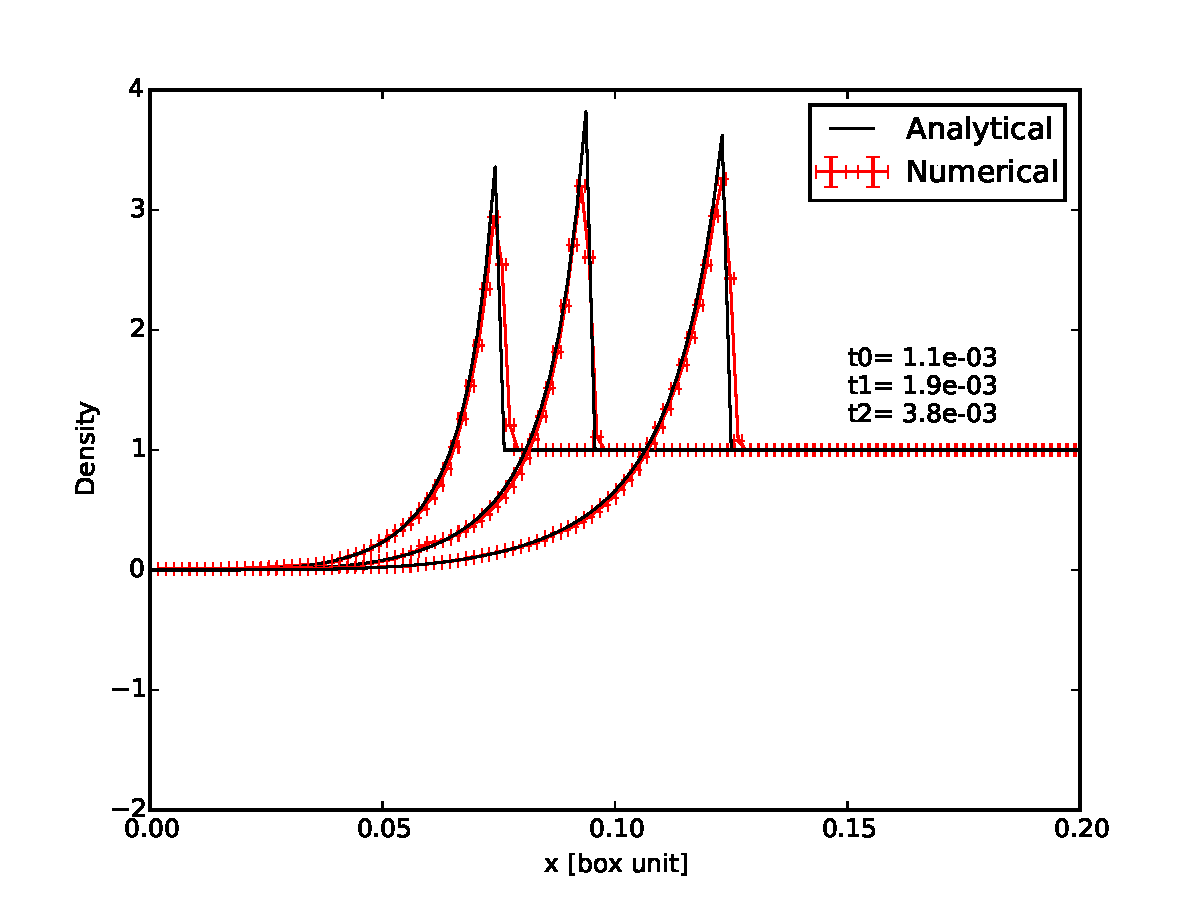
\includegraphics[width=\textwidth]{img/03/sedov/sedov_evol_8_den_lin.pdf} 
		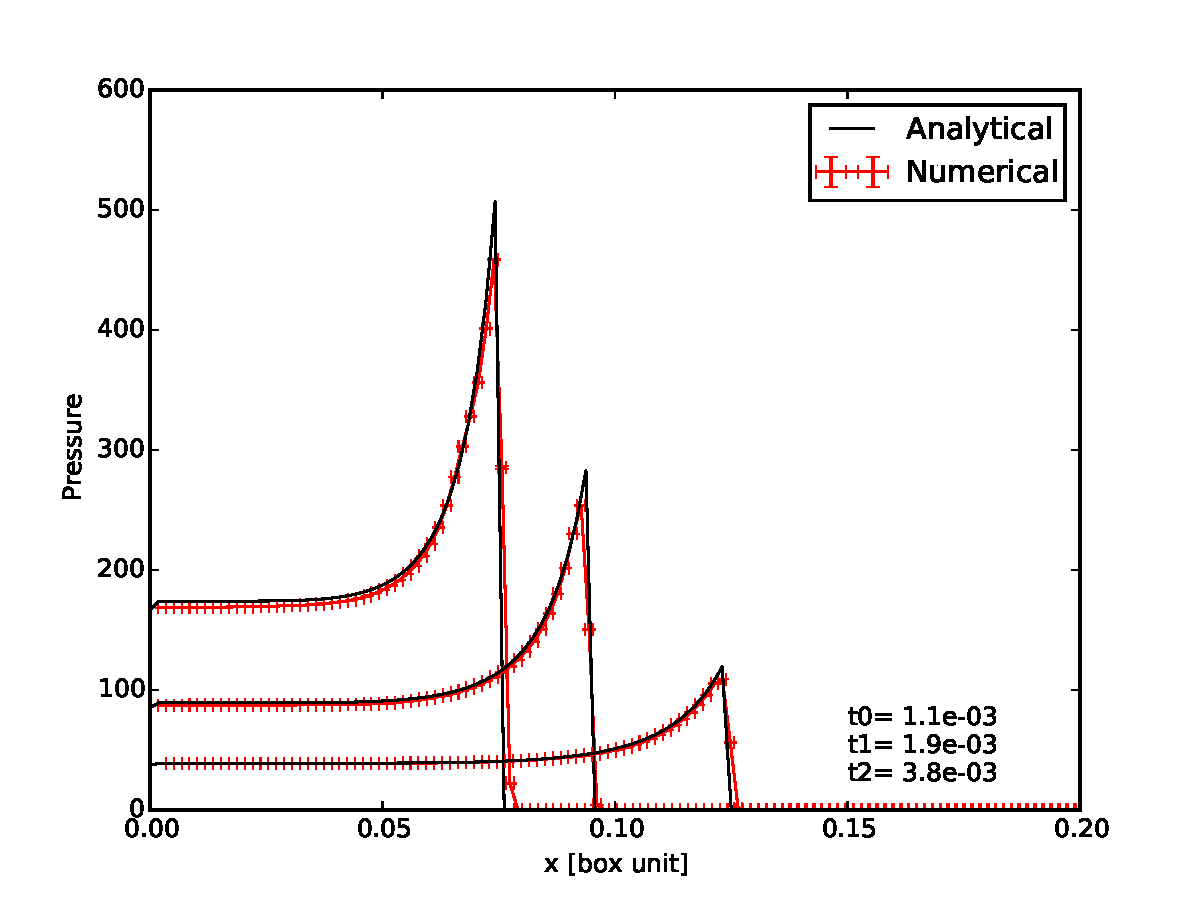
\includegraphics[width=\textwidth]{img/03/sedov/sedov_evol_8_pres.pdf} 
		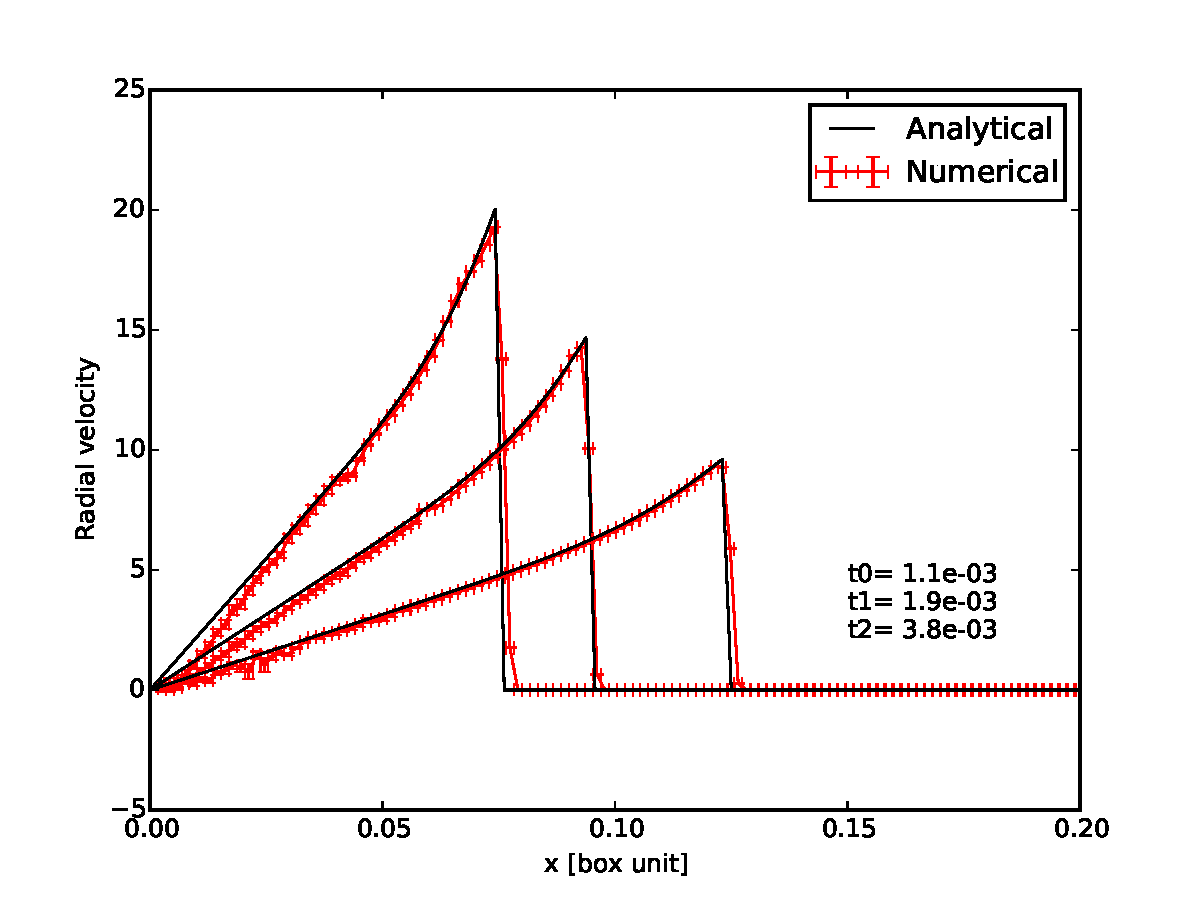
\includegraphics[width=\textwidth]{img/03/sedov/sedov_evol_8_vel.pdf} 

   \end{minipage} \hfill
   \begin{minipage}[c]{.5\linewidth}
		
		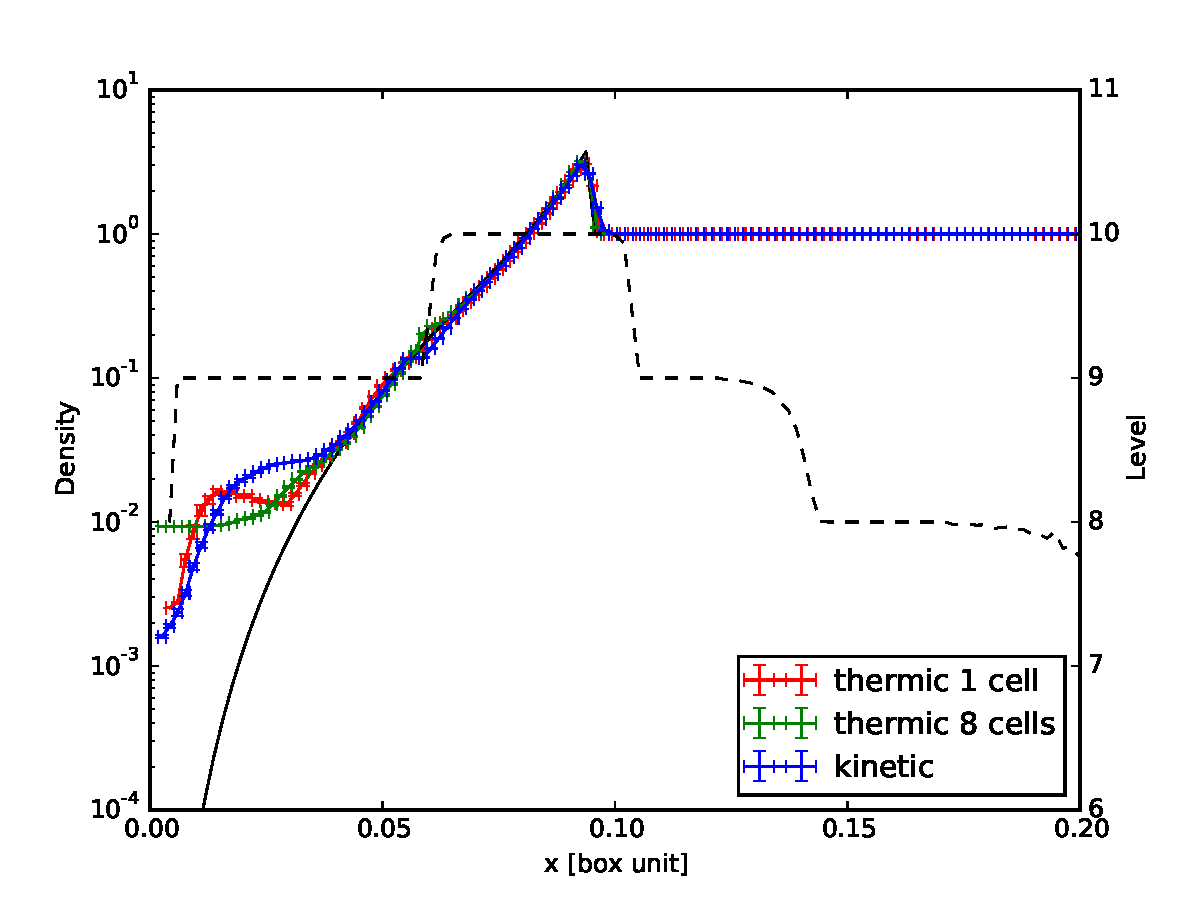
\includegraphics[width=\textwidth]{img/03/sedov/sedov_comp_profile_den.pdf} 
		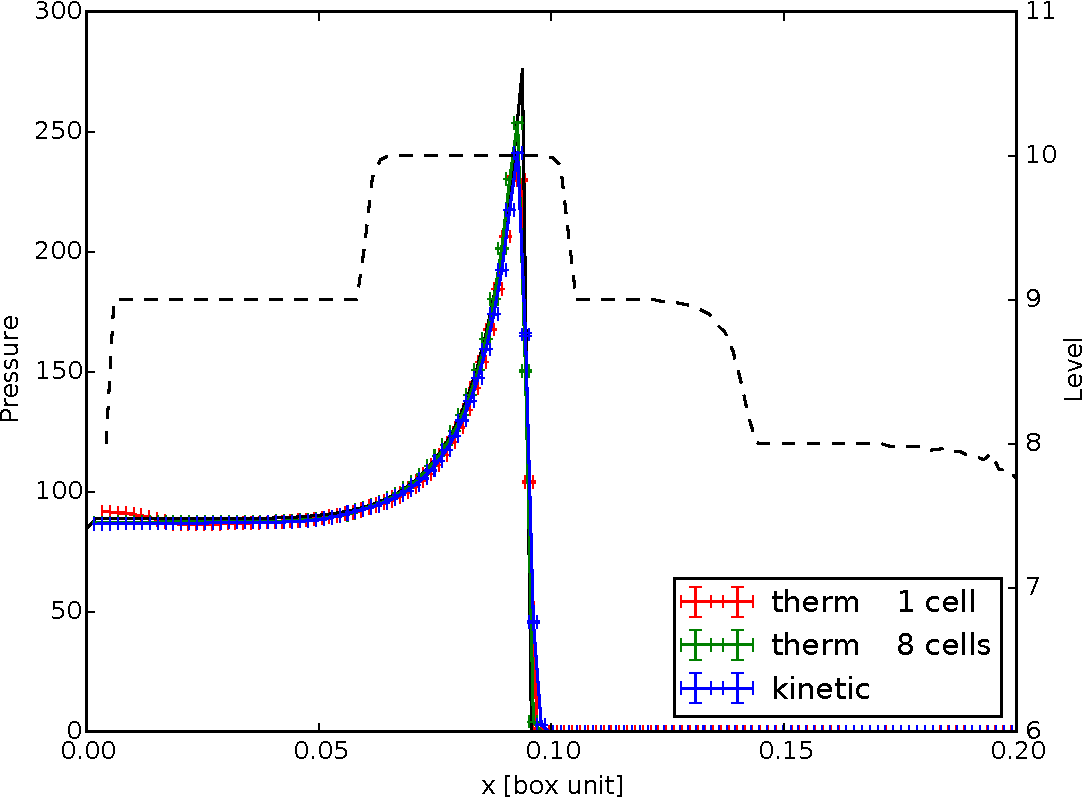
\includegraphics[width=\textwidth]{img/03/sedov/sedov_comp_profile_pres.pdf} 
		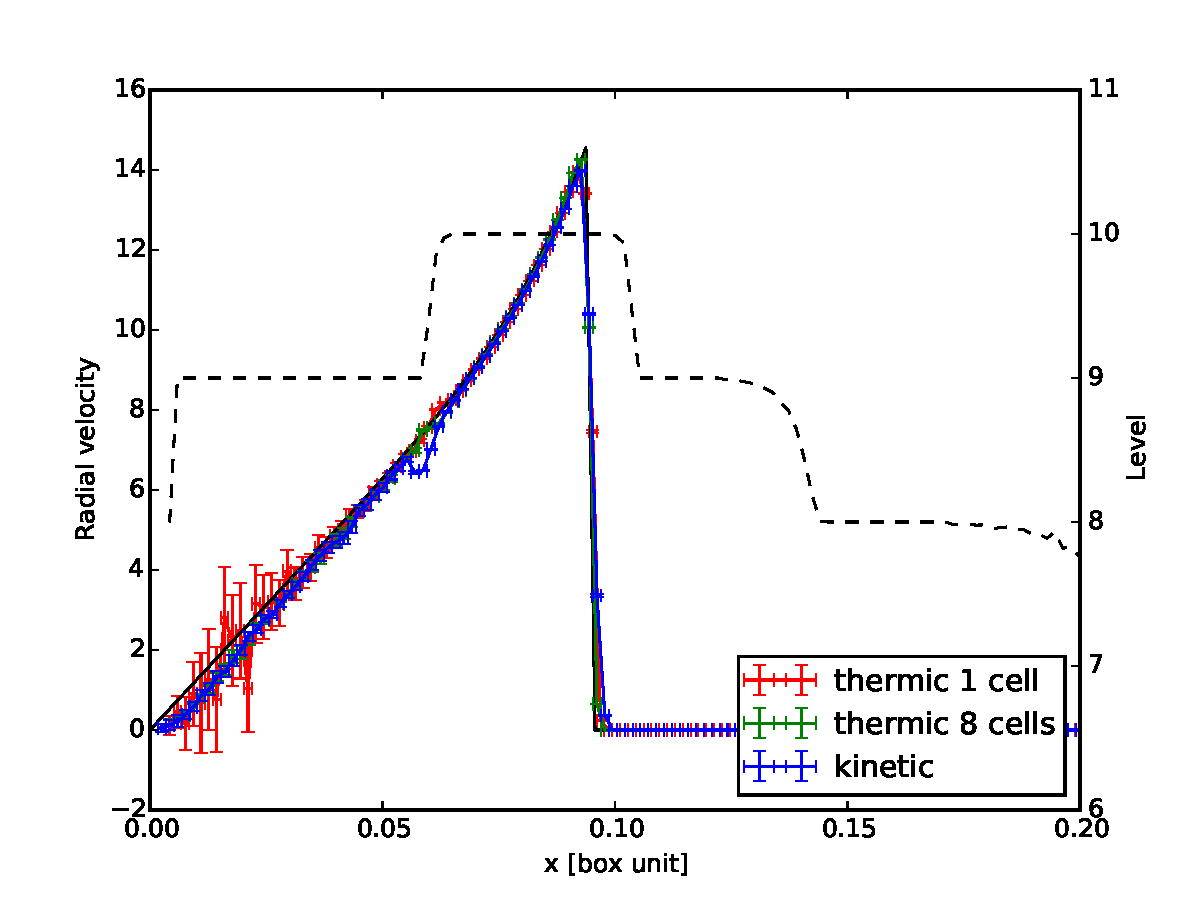
\includegraphics[width=\textwidth]{img/03/sedov/sedov_comp_profile_vel.pdf} 

   \end{minipage}

        \caption[Test de Sedov - Profils]{Profils radiaux des différentes variables d'états lors du test de Sedov, . 
        La densité en haut, la pression au milieu et la vitesse radiale en bas.     
        Colonne de gauche :
        Comparaison des profils à différents instants avec le méthode d'injection thermique.
        L'accord avec la théorie est excellent.
        Colonne de droite :    
        Comparaison en fonction des méthodes d'injection. 
        La position et la forme du front d'onde ne dépendent pas de la méthodes d'injection utilisée.
 		\label{fig:sedov_profil}
 		}
\end{figure}

\begin{figure}

	\centering
	\subfloat[]{ 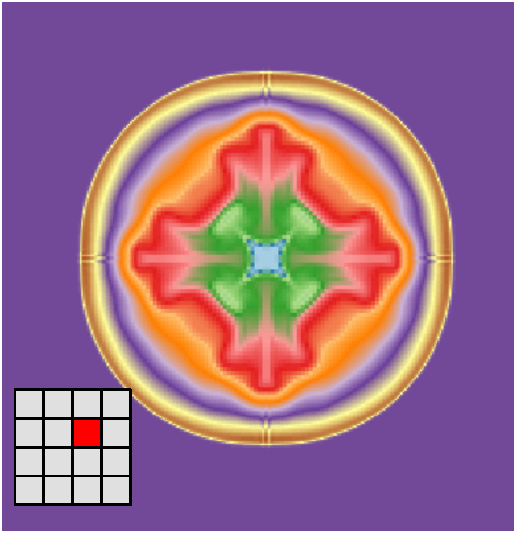
\includegraphics[width=.45\linewidth]{img/03/sedov/slice_therm1.pdf}} 
	\subfloat[]{	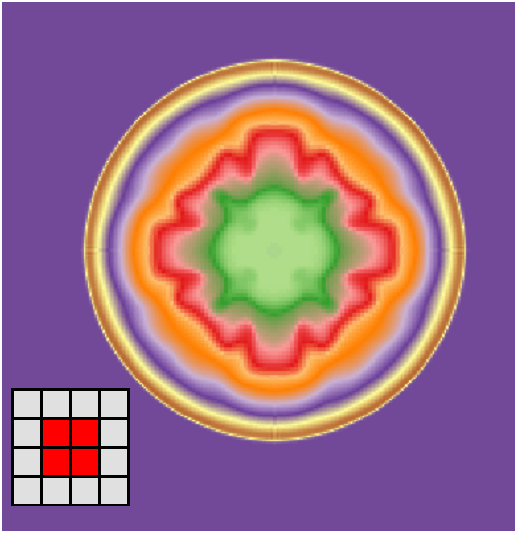
\includegraphics[width=.45\linewidth]{img/03/sedov/slice_therm4.pdf}} \\

	\subfloat[]{	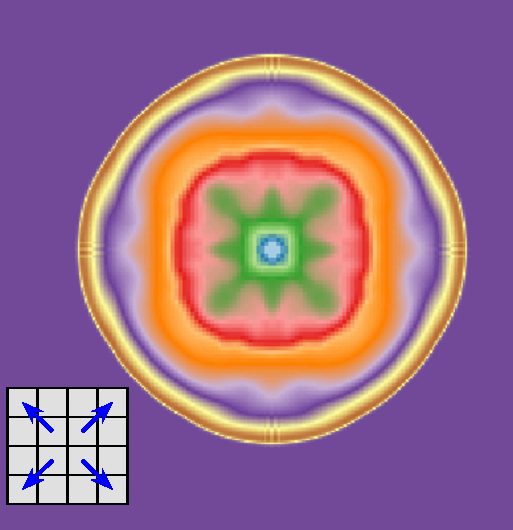
\includegraphics[width=.45\linewidth]{img/03/sedov/slice_kin.pdf} }
	\subfloat[]{	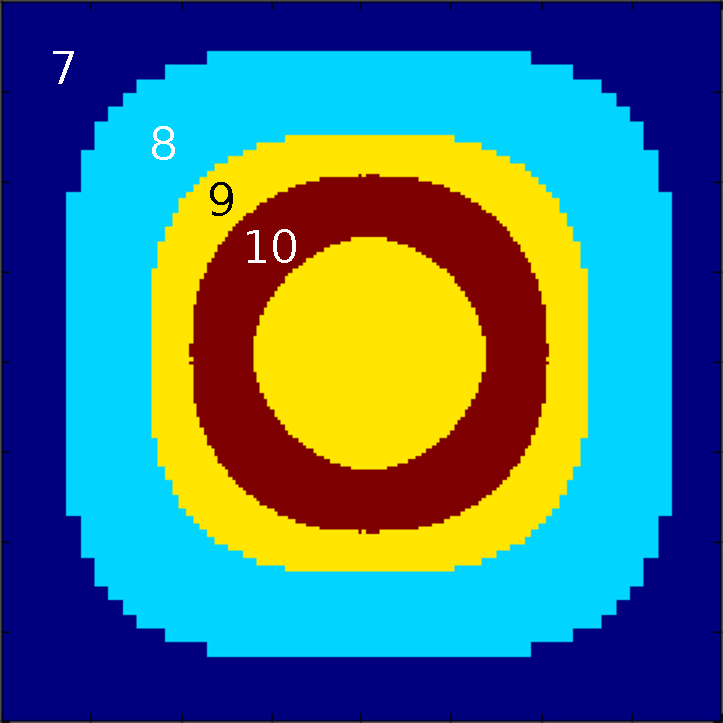
\includegraphics[width=.45\linewidth]{img/03/sedov/slice_th_1raf_cut.pdf}}

    \caption[Test de Sedov - Tranches]{Différents motif d'explosion en fonction de la méthodes d'injection.
    Chaque figure représente une tranche d'une cellule d'épaisseur contenant le site de l'explosion.
    (a), (b) et (c) représente le champ de densité prit au même instant.
    Dans le but d'accentuer les différence, la représentation utilise le logarithme de la densité avec une colormap quantitative.
    A cause de la grille de calcul, il existe des axes privilégiés pour les flux, il en résulte des motif en croix et ou en losange.
    La figure (d) représente les niveaux de raffinements, l'échelle est différente et le niveau 10 est aligné sur le front d'onde.
    }
 	\label{fig:sedovslice}
\end{figure}

\subsection{Calibration}
\label{sec:sncali}

La quantité d'énergie et de masse injectée est calibrée en utilisant les informations en sortie de Starburst99.
Dans EMMA le modèle actuel ne considère pas la possibilité d'une explosion continue, avec un retour de masse ou d'énergie s'étalant dans le temps.
L'injection est réalisée instantanément quand la quantité d’énergie théorique donnée par Starburt99 représente 50\% de l’énergie totale.
La comparaison entre les sorties de Starburst99 et le modèle implémenté est présenté sur la figure \ref{fig:SNloss}.
Dans ce modèle, un particule stellaire de $M=10^6 M_\odot$ injectera $E_{SN} = 9.7\cdot 10^{11} J.kg^{-1}$ et perdra 53\% de sa masse dans le milieu environnant, $17.6$ millions d'années après sa formation.
On notera l'injection de l'énergie apportée par les supernovae a lieu après un temps environ quatre fois plus grand que le temps de fin de vie radiatif ($t_{life} = 3.7$Myr).

De plus on introduira le rendement énergétique des supernovae $\epsilon_{SN}$, ce paramètre libre sera appliqué à $E_{SN}$ et sera utile pour calibrer l'impact de nos modèles.
A l'instar du paramètre de fraction d'échappement intrinsèque du rayonnement (cf section \ref{sec:etoilerad}) il contient une grande partie de la physique sous-grille qui n'est pas modélisée ici, comme la turbulence ou les champs magnétiques par exemple.

\begin{figure}
        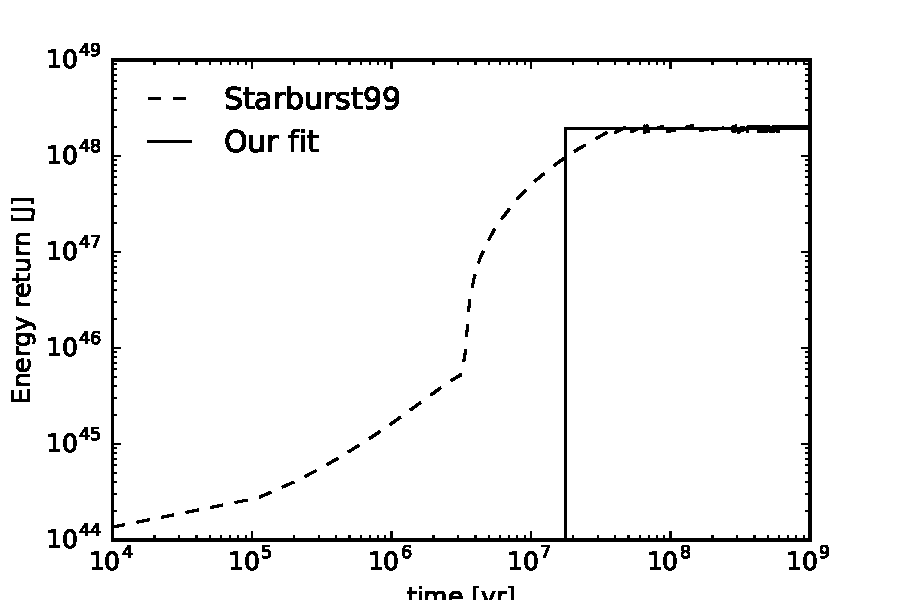
\includegraphics[width=.95\textwidth]{img/03/energy_loss.pdf} 
		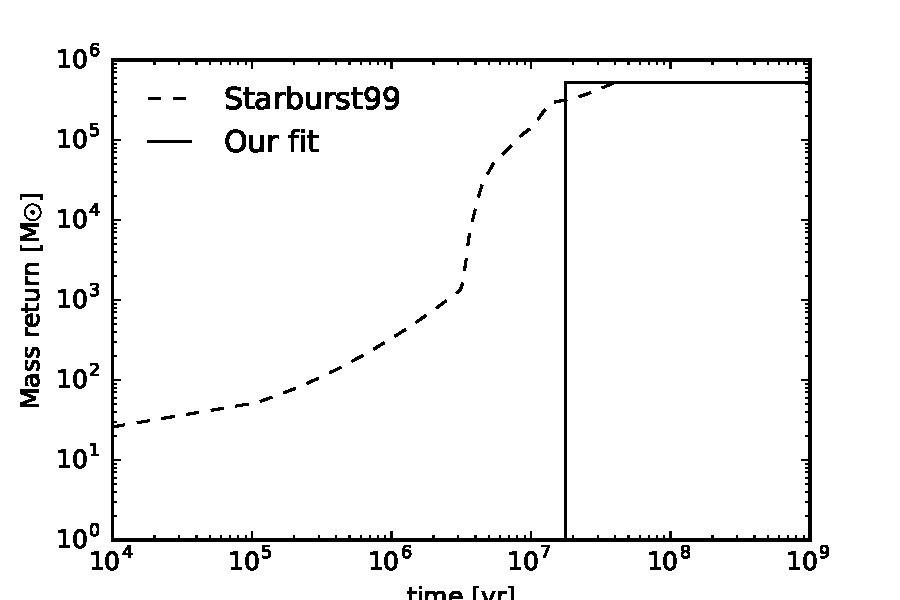
\includegraphics[width=.95\textwidth]{img/03/mass_loss.pdf} 
        \caption[Calibration des supernovæ]{ Quantité d'énergie et de masse injectés par les supernovae. 
        Comparaison entre le modèle théorique de Starburst99 et le modèle d'injection instantané implémenté dans EMMA.
 		\label{fig:SNloss}}
\end{figure}


\section{Tests du modèle en conditions de production}

L'objectif de cette section est de présenter quelques tests pour valider le modèle de formation et d'évolution stellaire développé dans les sections précédentes.
Dans un premier temps, j'ai réalisé une série de simulations, avec pour objectif d'obtenir une \ac{SFH} et un redshift de réionisation simulé en accord raisonnable avec les contraintes observationnelles.

%Dans le but de tester ces différentes méthodes d'injections dans un contexte cosmologique j'ai réalisé une série de simulations.
%\subsubsection{Présentation des simulations}
\subsection{Présentation des simulations}
\label{sec:pres_simu}

L'idée est d'étudier une série de simulations de taille relativement restreinte, servant d'échantillons, dans le but de mieux cerner l'impact du modèle stellaire dans les grandes simulations de la réionisation de type CoDa.
Ces échantillons ont la même résolution spatiale et massique que la simulation CoDa I - AMR (voir section \ref{sec:CODAEMMA}), et présentent l'avantage de pouvoir être exécutées en grand nombre et d'être bien plus manipulable.

Les paramètres communs à toutes les simulations qui vont suivre sont les suivants:
elles représentent un volume de $\left( 8\cdot h^{-1} \mathrm{cMpc} \right)^3$ échantillonné par $256^3$ éléments de résolution, % particules de matière noire.
ce qui mène à une résolution en masse de $3.4 \cdot 10^6 M_\odot$ et une résolution spatiale de $46$ckpc sur le niveau de base.
La grille est raffinée suivant une méthode semi-Lagrangienne (voir Sec. \ref{sec:raffinement}) avec une limite de résolution  physique de 1 kpc, menant à l'ajout de 3 niveaux supplémentaires à $z=6$.
Les condition initiales ont été générées avec MUSIC \citep{hahn_multi-scale_2011} avec une cosmologie de Planck \citep{planck_collaboration_planck_2016} : 
$\Omega_m=0.3175$, 
$\Omega_v=0.6825$,
$\Omega_b=0.0490$,
$H_0=67.11$,
$\sigma_8=0.830$. 
Les simulations commencent à redshift $z=150$ et s’arrêtent à $z=5$.

\subsection{Test de formation stellaire}

%le premier test réalisé consiste à comparer le \ac{SFR} cosmique de l'ensemble de la boite, aux observations.
Une difficulté est qu'il existe une dégénérescence entre le seuil en densité et l'efficacité de formation stellaire.
En effet, il semble à priori possible d'obtenir des résultats similaire en utilisant soit un seuil très permissif et une efficacité très faible, ou à l'inverse en ne formant des étoiles que dans les quelques cellules les plus denses avec une efficacité élevée.
Dans la littérature un seuil en surdensité de $\delta_{in}=50\bar{\rho}$ est régulièrement utilisé dans des simulations avec des résolutions comparables à celle-ci \citep{ocvirk_cosmic_2015,stinson_star_2006}.
L'utilisation d'un tel seuil en surdensité permet de bloquer simplement la formation stellaire à très haut redshift où le contraste de densité était faible.
J'ai donc fixé ce seuil et ajusté l'efficacité en conséquence.
Une valeur de $1\%$ à été retenue ici.
La figure \ref{fig:test_SFH} présente l'histoire de formation stellaire dans un volume de $\left( 8\cdot h^{-1} \mathrm{cMpc} \right)^3$ obtenue après calibration. 
Les contraintes observationnelles sont extraites de \cite{bouwens_reionization_2015}.
%une compilation réalisée par \cite{madau_cosmic_2014}.
Le couplage entre l'efficacité de formation stellaire et le feedback de supernovae est important (voir section \ref{sec:feedsfr}), donc pour minimiser ces effets de couplage entre les générations successives d'étoiles les supernovæ ne sont pas considérées ici.
Les premières étoiles apparaissent autour du redshift $z\approx 14$, contraint par le paramètre de surdensité.
On observe un saut dans la \ac{SFH} autour de redshift $z=10$ dû à l'enclenchement du dernier niveau de raffinement.

Avec ces paramètres, la \ac{SFH} obtenue respecte les contraintes observationnelles.
Cependant il faut garder à l'esprit que le volume physique représenté dans ces simulations étant relativement modeste et que la variance cosmique peut avoir un effet important sur la \ac{SFH}.
En effet, le volume étant restreint, une partie des halos massifs représentant une part non négligeable du \ac{SFR} total n'est pas présents dans ces simulations.
La réalisation de simulations représentant des volumes plus grands et avec des paramètres identiques, mène à une augmentation de la \ac{SFH} globale.
De plus, avec l'introduction des supernovae, les effets de rétroactions peuvent être importants rendant complexes les calibrations.
%Si la SFR est volontairement sous évaluée dans ces boites 
%C'est pourquoi il ne faut pas accorder trop d'importance à la reproduction des contraintes sur le taux de formation stellaire dans ces volumes.% cette contrainte prenant plus d'importance dans des volumes où la variété de 
C’est pourquoi nous visons dans ces volumes à une reproduction raisonnable des contraintes sans lui accorder non plus une importance démesurée.

\begin{figure}
        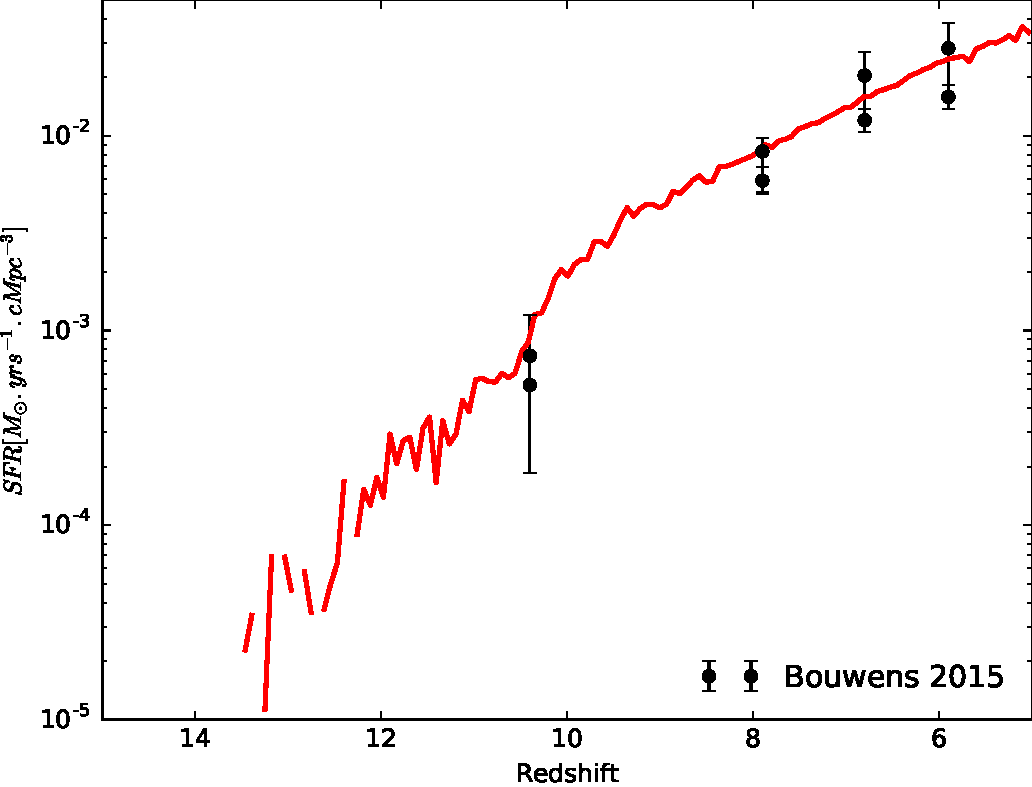
\includegraphics[width=.95\linewidth]{img/02/SFR.pdf}
        \caption[Histoire de formation stellaire]{Histoire de formation stellaire (SFH) d'une simulation de (8/h cMpc)$^3$.
        Il est possible d'obtenir une SFH qui respecte les observations avec un modèle relativement simple.
}
 		\label{fig:test_SFH}
\end{figure}

\subsection{Test d'ionisation}
Avec les paramètres déterminés par Starburst99 et une fraction d'échappement intrinsèque de 40\%, j'obtiens l'histoire de reionisation présenté sur la figure \ref{fig:test_xion}.
Cette histoire est comparable aux contraintes observationnelles déterminées par \cite{fan_constraining_2006}.
J'ai également pu vérifier à ce stade que l'introduction du rayonnement ionisant dans la simulation a peu d'impact sur la \ac{SFH} cosmique.
Ce qui permet de calibrer d'abord la \ac{SFH} puis ensuite l'émissivité des sources.

\begin{figure}
        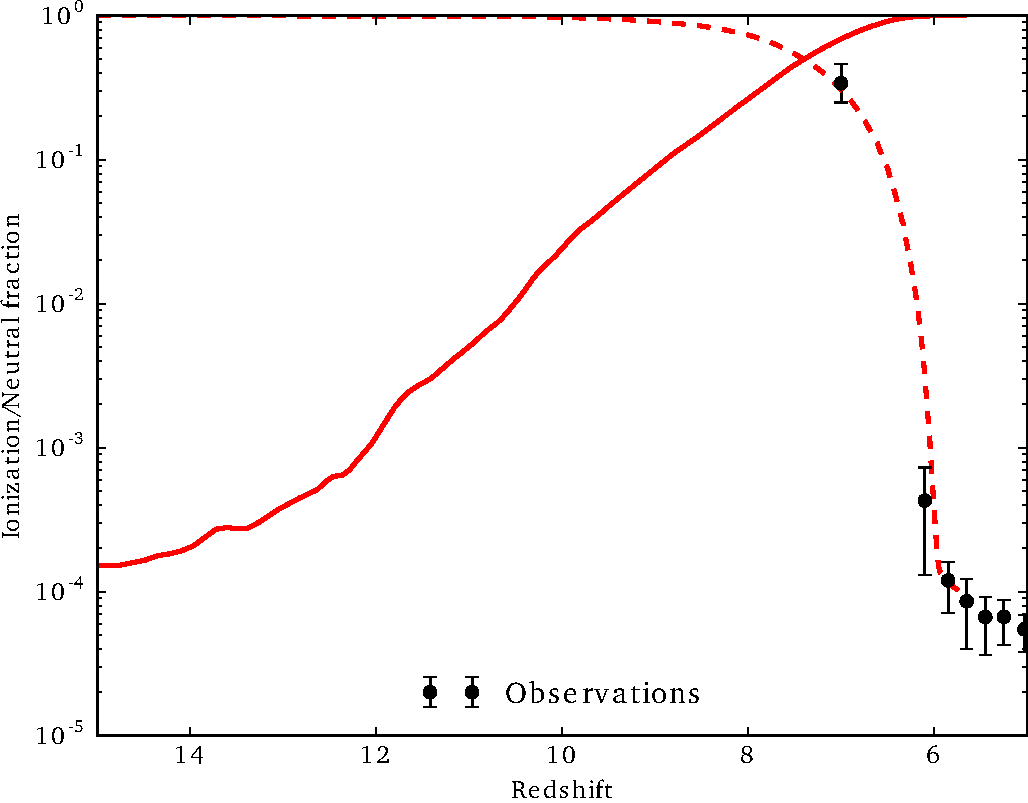
\includegraphics[width=.95\linewidth]{img/02/xion.pdf} 
        \caption[Histoire d'ionisation]{Évolution de la fraction d'ionisation (trais plein) et de la fraction de neutre (tirets) dans la simulation présentée sur la figure \ref{fig:test_SFH}.
        Après calibration de la fraction d’échappement intrinsèque, il est possible d'obtenir une histoire d'ionisation en accord avec les observations.
 		\label{fig:test_xion}}
\end{figure}

\subsubsection{Influence de la masse des particules stellaires}

%le paramètre de masse des étoiles change la reionization\\
%effet numérique\\
%le rayonnement est piégé dans les cellules\\

Durant mes calibrations, il s'est avéré que le paramètre de résolution de la masse des particules stellaire $m_{star}$ avait une grande importance dans l'évolution de la fraction ionisée.
Dans des simulations hydrodynamiques dédiées à l'étude de la formation des galaxies mais non spécialisées dans l'étude de l'\ac{EoR}, ce paramètre n'a que peu d'importance.
Il a une faible influence sur la formation stellaire globale (cf panneau de gauche de la figure \ref{fig:mstar}).
%Cependant une masse importante  définira la limite sur la résolution de la formation stellaire dans les petits halos.
Dans le cas de simulations considérant les effets des sources ionisantes lors de l'\ac{EoR}, ce paramètre aura également une influence sur la propagation du rayonnement.
Même si ce paramètre n'a pas d'impact sur le \ac{SFR} global, le taux d'ionisation moyen en est fortement dépendant (cf panneau de droite de la figure \ref{fig:mstar}).
Les "grosses" particules stellaire mènent à un taux d'ionisation plus important.
À l'inverse, plus la résolution stellaire est élevée, plus la boite réionise tard.
Il s'agit ici d'un effet numérique: pour les plus petites particules stellaires le rayonnement se trouve piégé au sein des cellules les plus denses en gaz.
Pour les petites particules, le rayonnement est dilué à la fois dans l'espace et dans le temps, alors que dans le cas d'une grosse particule, une grosse quantité de rayonnement est injectée à un instant donné, la cellule est flashée et le rayonnement peut s'échapper.
La difficulté sera de trouver un compromis entre :

\begin{itemize}
\item particules stellaires massives, permettant au rayonnement de sortir facilement des cellules au détriment d'une mauvaise résolution sur la formation stellaire
\item  et particule stellaire de faible masse, générant une formation stellaire résolue même dans les petits halos mais menant à une réionisation plus difficile et une occupation mémoire plus importante.
De plus, si la masse devient trop faible, les particules ne sont plus statistiquement représentative d'une population.
Dans les cas extrêmes, il pourrait devenir nécessaire de former des étoiles individuellement, en échantillonnant les masses individuellement partir d'une \ac{IMF}.
\end{itemize}

Dans la suite de cette étude, les étoiles seront relativement massives puisque $m_* \approx 7.7 \cdot 10^4 M_\odot$.


\begin{figure}
        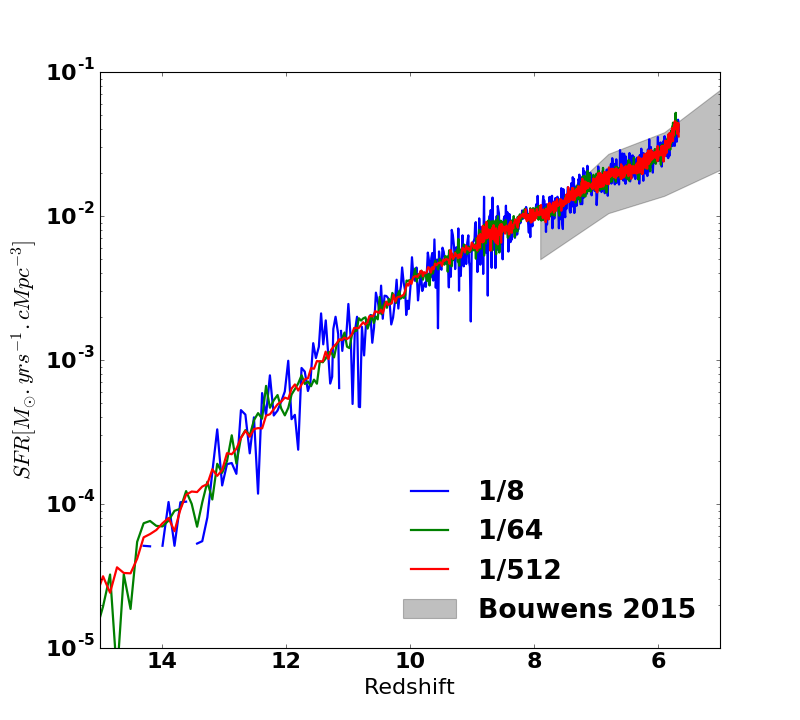
\includegraphics[width=.5\textwidth]{img/02/Mstar_SFH.png} 
        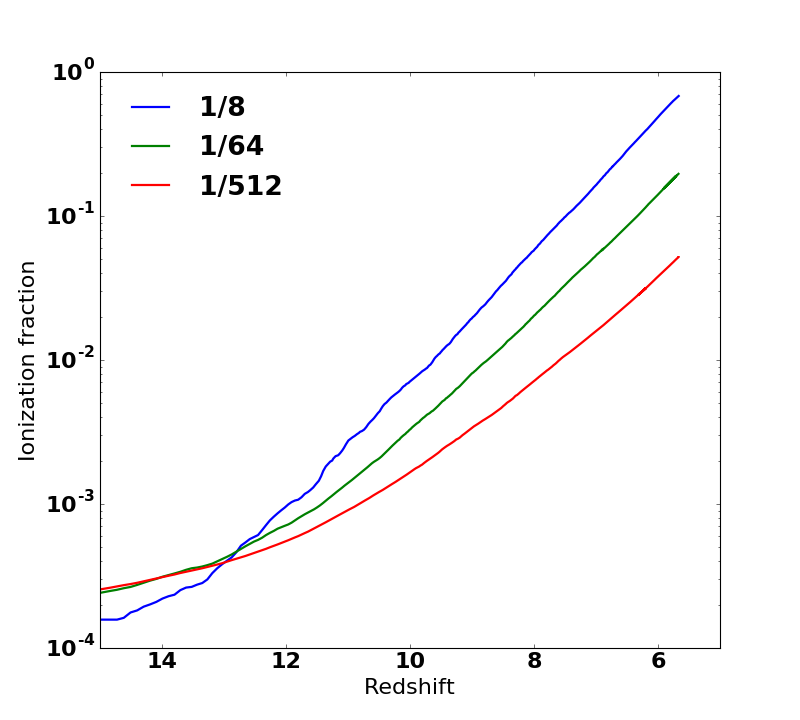
\includegraphics[width=.5\textwidth]{img/02/Mstar_xion.png} 
        \caption[Masses des étoiles]{En changeant le paramètre de résolution en masse des particules stellaire, la \ac{SFH} cosmique moyenne reste constante mais l'histoire d'ionisation s'en trouve impactée.
 		\label{fig:mstar}}
\end{figure}

\clearpage
\subsection{Tests du modèle de supernovæ}
\label{sec:testsncosmo}

\subsubsection{Influence de la méthode d'injection}
\label{sec:snmethod}

Le premier test consiste à essayer les différents modèles de feedback avec la même quantité d'énergie injectée, et à mesurer leurs impacts respectifs sur la \ac{SFH} cosmique.
Toutes les simulations qui vont suivre sont strictement identiques à l'exception de la méthode d'injection d'énergie.
La figure \ref{fig:sfr_methode} présente les résultats obtenus avec quatre simulations.
Parmi ces simulations, il y en a :
\begin{itemize}
\item une sans rayonnement ni supernovae (NoFEED),
\item une sans supernovae (NoSN),
\item une avec supernovae - modèle thermique (Thermal),
\item une avec supernovae - modèle cinetique (Kinetic).
\end{itemize}

Alors que les deux méthodes présentent des résultats similaires dans le cas idéal, la méthode d'injection cinétique a plus d'impact en conditions cosmologiques.
À redshift $z=6$, la méthode d'injection thermique diminue le \ac{SFR} de moins d'un facteur 2 par rapport à la simulation sans radiation ni supernovæ, alors que la méthode cinétique le diminue d'un facteur environ 3.
Ceci est du à l'introduction de la physique du refroidissement.
La méthode thermique repose sur le principe de conversion de l'énergie interne en énergie cinétique, et le refroidissement limite cette conversion en permettant d'importantes pertes par rayonnement.
La méthode thermique est connue \citep{navarro_simulations_1993} pour subir d'importantes pertes d'énergie.
La méthode cinétique outre-passe cette conversion et met directement le gaz en mouvement.
Nous aurons donc tendance préférer la méthode cinétique par la suite, vu que celle ci est plus efficace pour mettre le gaz en mouvement à nos échelles.

%TODO parler du feedback radiatif

\begin{figure}
        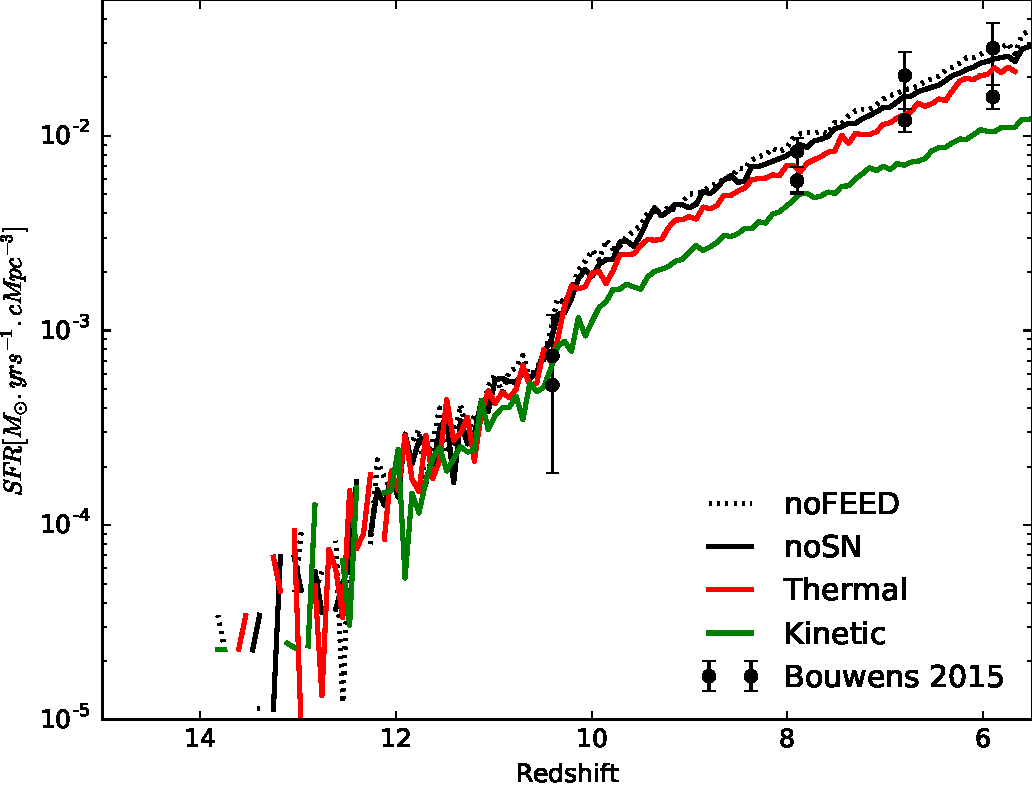
\includegraphics[width=.95\textwidth]{img/03/sedov/SFRmethode.pdf} 
        \caption[SFH cosmique en fonction de la méthode d'injection d'énergie]{SFH cosmique en fonction de la méthode d'injection d'énergie.
        Contrairement au test de Sedov, les différents méthodes n'impactent pas le milieu de la même manière.
        }
 		\label{fig:sfr_methode}
\end{figure}



\subsubsection{Influence de la quantité d'énergie injectée}
\label{sec:snegy}

Le deuxième test consiste à utiliser la méthode cinétique et à varier la quantité d'énergie injectée via le paramètre $\epsilon_{SN}$.
La figure \ref{fig:sfr_egy} présente les résultats obtenus.
On y observe que plus on injecte d'énergie, plus le \ac{SFR} instantané diminue.
Ce qui est le comportement attendus puisque plus les supernovae sont puissantes, plus les sur-densités de gaz sont "cassées", et donc il devient plus difficile de former de nouvelles étoiles.

\begin{figure}
        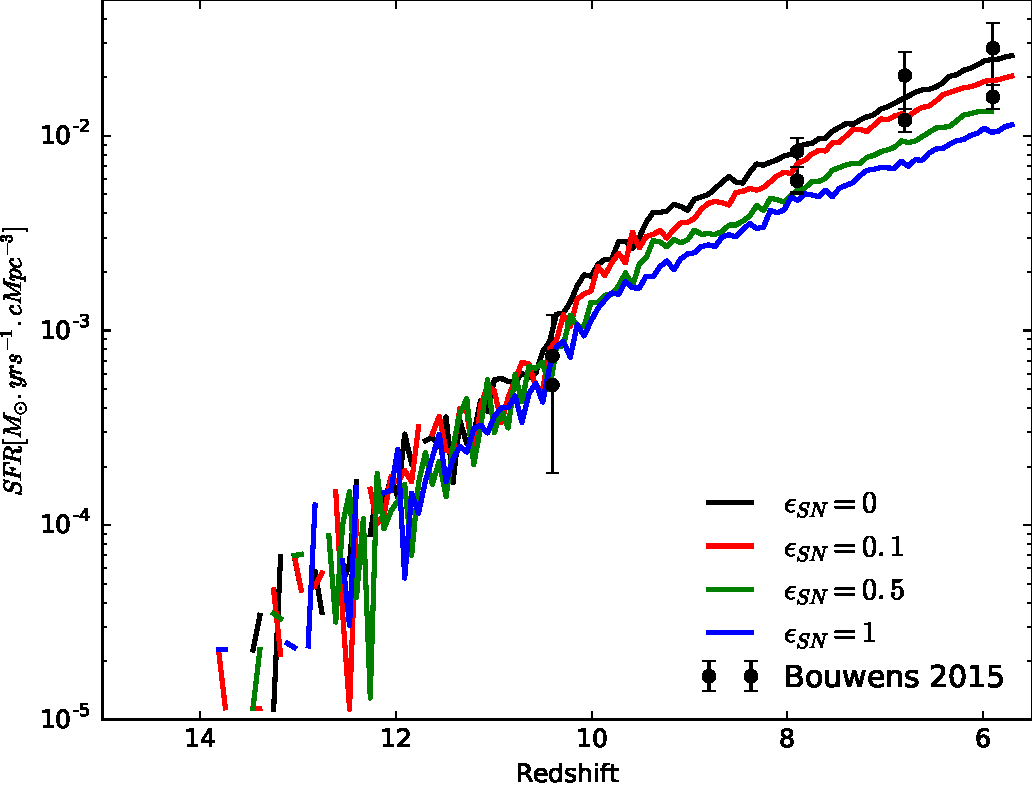
\includegraphics[width=.95\textwidth]{img/03/sedov/sneff_SFR.pdf} 
        \caption[SFH cosmique en fonction de la quantité d'énergie injectée]{SFH cosmique en fonction de la quantité d'énergie injectée. 
        Plus la quantité d'énergie injecté est importante, plus le taux de formation stellaire diminue.
        }
 		\label{fig:sfr_egy}
\end{figure}

\subsubsection{Couplage entre feedback et efficacité de formation stellaire}
\label{sec:feedsfr}

Le couplage entre feedback et formation stellaire n'est pas clair et mérite d'être exploré.
En effet, plus on forme d'étoiles et plus le feedback devient important, mais plus il y a de feedback, moins il est facile de former de nouvelles étoiles.

Le troisième test consiste à injecter une quantité donnée d'énergie par supernovae, et à faire varier l'efficacité de formation stellaire.
L'idée est de tester si la diminution du \ac{SFR} observée lors de l'injection d'énergie peut être compensée par l'augmentation de l'efficacité de formation stellaire.
La figure \ref{fig:sfr_sfe} présente ce test pour trois efficacités de formation stellaire différentes, avec un modèle de feedback cinétique et un rendement énergétique de supernovae de $\epsilon_{SN}=100$ \%.
On observe un fort couplage entre feedback et formation stellaire, à tel point que pour une efficacité de formation stellaire de 10\% le feedback mène à une \ac{SFH} décroissante.
A feedback donné et pour le volume considéré il n'est donc pas possible de remonter arbitrairement le \ac{SFR} en augmentant l'efficacité de formation stellaire, ce qui limite la dégénérescence entre ces deux paramètres.

\begin{figure}
        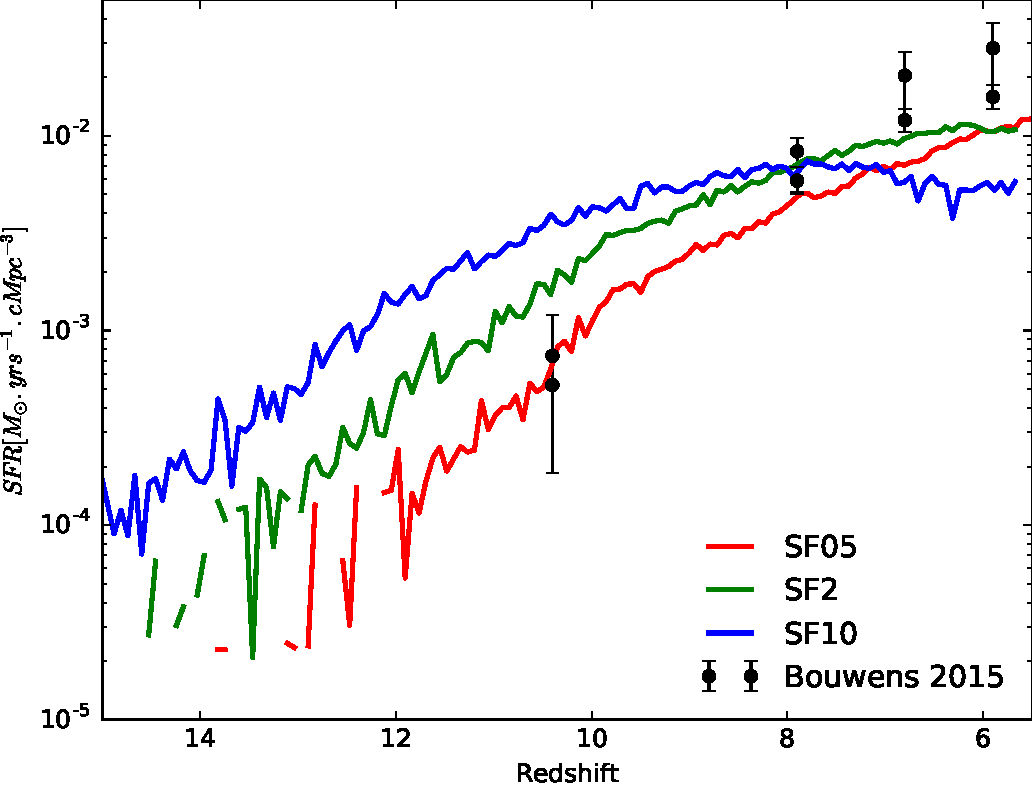
\includegraphics[width=.95\textwidth]{img/03/sedov/SFR_sfeff.pdf} 
        \caption[SFH cosmique en fonction de l'efficacité de formation stellaire]{SFH cosmique en fonction de l'efficacité de formation stellaire.
        Toutes les simulations utilisent la même méthode d'injection et la même quantité d'énergie.
		L'effet du couplage est bien présent.
        }
 		\label{fig:sfr_sfe}
\end{figure}





%\subsubsection{Conclusion}
%
%La conclusion de ses tests est que les différentes méthodes d'injection sont équivalentes, au moins dans le contexte du test de Sedov.
%OK\\
%mais pas en cosmo
%le pas de temps\\